% Paquets généraux
\documentclass[a4paper,12pt,titlepage,twoside]{article}
\usepackage[T1]{fontenc}
\usepackage[utf8]{inputenc}
\usepackage[french]{babel}
\usepackage{subcaption}
\addto\captionsfrench{%
  \renewcommand{\tablename}{Tableau}%
}
\usepackage[gen]{eurosym}
%\usepackage[dvips]{graphicx}
\usepackage{minted}
\usepackage{fancyhdr}
\usepackage{pdfpages} 
\usepackage{multido}
\usepackage{hyperref}
\usepackage{textcomp}
\usepackage{schemabloc}
%\usepackage[bitstream-charter]{mathdesign}
\usepackage{array}
\newcolumntype{P}[1]{>{\centering\arraybackslash}p{#1}}
\usepackage[shortlabels]{enumitem}
\usepackage[framemethod=TikZ]{mdframed}

\newcommand{\id}{71}
\newcommand{\nom}{Théorie des mécanismes}
\newcommand{\sequence}{04}
\newcommand{\nomsequence}{Liaisons entre les solides}
\newcommand{\num}{02}
\newcommand{\type}{KH}
\newcommand{\descrip}{Liaisons équivalentes, hyperstatisme, liaisons en série et en parallèle, théorie des graphes}
\newcommand{\competences}{B2-12: Proposer une modélisation des liaisons avec leurs caractéristiques géométriques. \\ &  B2-13: Proposer un modèle cinématique paramétré à partir d'un système réel, d'une maquette numérique ou d'u \\ &  B2-17: Simplifier un modèle de mécanisme. \\ &  B2-18: Modifier un modèle pour le rendre isostatique. \\ &  C1-04: Proposer une démarche permettant d'obtenir une loi entrée-sortie géométrique.  \\ &  C2-05: Caractériser le mouvement d'un repère par rapport à un autre repère. \\ &  C2-06: Déterminer les relations entre les grandeurs géométriques ou cinématiques. }
\newcommand{\nbcomp}{7}
\newcommand{\systemes}{}
\newcommand{\systemesnum}{}
\newcommand{\systemessansaccent}{}
\newcommand{\ilot}{2}
\newcommand{\ilotstr}{02}
\newcommand{\dossierilot}{\detokenize{Ilot_02 }}

%\usepackage{style}
\usepackage{bodegraph}
\usepackage{rpcinematik}
\usepackage[locale = FR]{siunitx}
\usepackage{caption}
\newcommand{\institute}{Lycée Dorian}

\usepackage{listings}
\usepackage{fancyvrb}
\usepackage{color}
\usepackage{xcolor}
\usepackage{colortbl}
\usepackage{helvet}
\usepackage[frenchmath]{newtxsf} % for sans serif symbols
\renewcommand{\familydefault}{\sfdefault}
%\usepackage{amsfonts}
%\usepackage{amsmath}
%\usepackage{lmodern}
\usepackage{mathastext}
%\usepackage{xspace}
\usepackage{varioref}
\usepackage{tabularx}
%\usepackage{floatflt}
\usepackage{graphics}
\usepackage{wrapfig}
\usepackage{textcomp}
\usepackage{tikz,tkz-tab}
\usepackage[european resistor, european voltage, european current]{circuitikz}
\usepackage{wrapfig}
\usepackage{gensymb}
\usepackage[percent]{overpic}
\usetikzlibrary{babel}
\usepackage{ifthen}
\usepackage{cancel}
\usepackage{etoolbox}
\usepackage{multirow}
%\usepackage{boxedminipage}
\definecolor{gris25}{gray}{0.75}
\definecolor{bleu}{RGB}{18,33,98}
\definecolor{bleuf}{RGB}{42,94,171}
\definecolor{bleuc}{RGB}{231,239,247}
\definecolor{bleum}{RGB}{160,195,226}
\definecolor{rougef}{RGB}{185,18,27}
\definecolor{rougec}{RGB}{255,188,204}%255,230,231
\definecolor{vertf}{RGB}{103,126,82}
\definecolor{vertc}{RGB}{220,255,191}
\definecolor{forestgreen}{rgb}{0.13,0.54,0.13}
\definecolor{blcr}{rgb}{0.59,0.69,0.84}
\definecolor{blfr}{rgb}{0.32,0.51,0.75}
\definecolor{orfr}{rgb}{0.90,0.42,0.15}
\definecolor{orcr}{rgb}{0.90,0.65,0.50}
\definecolor{orangef}{rgb}{0.659,0.269,0.072}
\definecolor{orange}{rgb}{0.58,0.35,0.063}
\definecolor{orangec}{rgb}{0.43,0.32,0.25}
\definecolor{rcorrect}{rgb}{0.6,0,0}
\definecolor{sequence}{rgb}{0.75,0.75,0.75}
\definecolor{competences}{rgb}{0.61,0.73,0.35}
\definecolor{rose}{HTML}{ff00ff}
\definecolor{grisf}{HTML}{222222}
\definecolor{grisc}{HTML}{636363}
\definecolor{normal}{HTML}{4087c4}
\definecolor{info}{HTML}{5bc0de}
\definecolor{success}{RGB}{92,184,92}
\definecolor{warning}{RGB}{240,173,78}
\definecolor{danger}{RGB}{217,83,79}
\hypersetup{                    % parametrage des hyperliens
    colorlinks=true,                % colorise les liens
    breaklinks=true,                % permet les retours à la ligne pour les liens trop longs
    urlcolor= blfr,                 % couleur des hyperliens
    linkcolor= orange,                % couleur des liens internes aux documents (index, figures, tableaux, equations,...)
    citecolor= forestgreen                % couleur des liens vers les references bibliographiques
    }

\newcolumntype{M}[1]{>{\centering\arraybackslash}m{#1}}
\definecolor{codegreen}{rgb}{0,0.6,0}
\definecolor{codegray}{rgb}{0.5,0.5,0.5}
\definecolor{codepurple}{rgb}{0.58,0,0.82}
\definecolor{backcolour}{rgb}{0.95,0.95,0.92}

\lstdefinestyle{mystyle}{
    backgroundcolor=\color{backcolour},   
    commentstyle=\color{codegreen},
    keywordstyle=\color{magenta},
    numberstyle=\tiny\color{codegray},
    stringstyle=\color{codepurple},
    basicstyle=\ttfamily\footnotesize,
    breakatwhitespace=false,         
    breaklines=true,                 
    captionpos=b,                    
    keepspaces=true,                 
    numbers=left,                    
    numbersep=5pt,                  
    showspaces=false,                
    showstringspaces=false,
    showtabs=false,                  
    tabsize=2
}

\lstset{style=mystyle}

% Mise en page
\pagestyle{fancy}

\setlength{\hoffset}{-18pt}
\setlength{\oddsidemargin}{0pt} 	% Marge gauche sur pages impaire2s
\setlength{\evensidemargin}{0pt} 	% Marge gauche sur pages paires
\setlength{\marginparwidth}{00pt} 	% Largeur de note dans la marge
\setlength{\headwidth}{481pt} 	 	% Largeur de la zone de tête (17cm)
\setlength{\textwidth}{481pt} 	 	% Largeu\textbf{r de la zone de texte (17cm)
\setlength{\voffset}{-18pt} 		% Bon pour DOS
\setlength{\marginparsep}{7pt}	 	% Séparation de la marge
\setlength{\topmargin}{-30pt} 		% Pas de marge en haut
\setlength{\headheight}{55pt} 		% Haut de page
\setlength{\headsep}{20pt} 		% Entre le haut de page et le texte
\setlength{\footskip}{30pt} 		% Bas de\textbf{ page + séparation
\setlength{\textheight}{700pt} 		% Hauteur de l'icone zone de texte (25cm)
\setlength\fboxrule{1 pt}
\renewcommand{\baselinestretch}{1}
\setcounter{tocdepth}{1}
\newcommand{\cadre}[2]
{\fbox{
  \begin{minipage}{#1\linewidth}
   \begin{center}
    #2\\
   \end{center}
  \end{minipage}
 }
}

\newcommand{\repon}[1]
{
~\ \\
\begin{tabular}{|m{\linewidth}|}
 \hline
\multido{}{#1}{\\ \hline}
\end{tabular}
}


\newcommand{\objectif}[1]{
\mdfsetup{%
frametitle={%
\tikz[baseline=(current bounding box.east),outer sep=0pt]
\node[anchor=east,rectangle,fill=bleum]
{\strut Objectif~};}}
\mdfsetup{innertopmargin=10pt,linecolor=bleum,%
linewidth=2pt,topline=true,%
frametitleaboveskip=\dimexpr-\ht\strutbox\relax
}
\begin{mdframed}[]\relax%
#1
\end{mdframed}}


\newcounter{num_quest} \setcounter{num_quest}{0}
\newcounter{num_rep} \setcounter{num_rep}{0}
\newcounter{num_cor} \setcounter{num_cor}{0}

\newcommand{\feuilleDR}[1]{
	\begin{tikzpicture}
		\draw[gray!30](0,0)grid[step=0.5cm](\linewidth,#1);
	\end{tikzpicture}
}

%\newcommand{\question}[1]{\refstepcounter{num_quest}\par
%~\ \\ \parbox[t][][t]{0.15\linewidth}{\textbf{Question \arabic{num_quest}}}\parbox[t][][t]{0.85\linewidth}{#1\label{q\the\value{num_quest}}}\par
%}

\newcommand{\question}[1]{\refstepcounter{num_quest}\par
~\ \\ \textbf{Question \arabic{num_quest} : }#1\label{q\the\value{num_quest}}\par
}

\newcommand{\posetafigure}[3]{
\begin{figure}[ht!]
 \begin{center}
  \includegraphics[width=#2\linewidth]{img/#1}
 \end{center}
 \caption{\label{#1} #3}
\end{figure}}

\newcommand{\goforum}{
\begin{figure}

\end{figure}
\begin{center}
 
\includegraphics[width=0.7\linewidth]{../../../img/go_forum}
\end{center}
\label{go_forum}
\caption{J'pète les plombs}
\end{figure}}

\newcommand{\reponse}[4][1]
{\noindent
\parbox{\textwidth}{
\rule{\linewidth}{.5pt}\\
\textbf{Question\ifthenelse{#1>1}{s}{} \multido{}{#1}{%
\refstepcounter{num_rep}\ref{q\the\value{num_rep}} }:} ~\ \\
\ifdef{\public}{#3 \ifthenelse{#2>0}{~\ \\ 	\feuilleDR{#2}}}{#4}
}}

\newcommand{\cor}
{\refstepcounter{num_cor}
\noindent
\rule{\linewidth}{.5pt}
\textbf{Question \arabic{num_cor}:} \\
}

\newcommand{\finsujet}
{
    \begin{center}
    \Large{FIN}
    \end{center}

    \cleardoublepage

    \ifdef{\public}{\pagestyle{docreponse}}{\pagestyle{correction}}

    \ifdef{\public}{
        \begin{tikzpicture} 
            \draw (0,0) rectangle (2,2);
            \draw (0,0) -- (2,2);
            \draw (1.5,0.5) node {\large 20};
            \draw (2.5,0) rectangle (16,2);
            \draw (4.5,1.7) node {\large Commentaires:};
        \end{tikzpicture}
    }
    ~\ \\
}


%\newcommand{\repcarre}[2]
%{
%~\ \\
%\begin{tikzpicture}
%\draw [fill=white] (0,0) rectangle +(\linewidth,#1);
%\node[align=left] at (1.1,#2-0.3) {\textbf{Question #1:}};
%\end{tikzpicture}
%}

\newcommand{\titre}[1]
{\begin{center}
\cadre{0.8}{\huge #1} 
\end{center}
}


%Définition des torseurs :
\newcommand{\torseur}[2]{\left\{\mathcal{#1}_{#2} \right\}}
\newcommand{\torseurh}[3]{\left\{\genfrac{}{}{0pt}{0}{#1}{#2}\right\}_{#3}}
\newcommand{\torseurv}[8]{\left\{
\begin{matrix}
#1 & #4 \\ #2 & #5 \\ #3 &#6
\end{matrix}
\right\}_{{#7},{#8}}}

%Définition des torseurs :
%\newcommand{\torseur}[2]{\left \{\mbox{\relsize{2}{$\mathcal {#1}$}\relsize{-2}}\phantom{}_{\mbox{\scriptsize $#2$}} \right \}}
%\newcommand{\torseurh}[3]{\left\{\genfrac{}{}{0pt}{0}{#1}{#2}\right\}_{#3}}
%\newcommand{\torseurv}[8]{
%\left\{\begin{array}{@{}c|c@{}} #1 & #4 \\ #2 & #5 \\ #3 & #6 \end{array} \right\}_{#7,#8}
%}
\newcommand{\derivee}[2]{\left.\dfrac{\d #1}{\d t}\right|_{#2}}
\newcommand{\tripleint}{\int\!\!\!\!\!\int\!\!\!\!\!\int}

% Notation cinématique et statique
\newcommand{\cinematique}[2]{\mbox{#1}/\mbox{#2}}
\newcommand{\statique}[2]{\mbox{#1}\rightarrow\mbox{#2}}
\newcommand{\moment}[3]{\vv {#1}_{\scriptsize{#3}}(#2)}
\newcommand{\resultante}[2]{\vv {#1}_{\scriptsize{#2}}}


%Commande de base
\newcommand{\jo}{\left(j\omega\right)} % j \omega dans l'analyse fréquentielle
\newcommand{\tl}{\xrightarrow{\mathcal{L}}} % transformée de laplace sur fleche
\newcommand{\tli}{\xrightarrow{\mathcal{L}^{-1}}} % transformée inverse de laplace sur fleche
\renewcommand{\d}[1][]{\mathrm{d#1}}
\newcommand{\dd}[1][]{\mathrm{d#1}}
\newcommand{\vect}[2]{{#1}\wedge{#2}}
\newcommand{\base}[3]{(\vec #1,\vec #2,\vec #3)}
\newcommand{\vectbase}[4]{{\vphantom{\left| \begin{matrix}
#1\\#2\\#3 \end{matrix} \right|}}_{#4}{\left| \begin{matrix}
#1\\#2\\#3 \end{matrix} \right.}}
%Pour avoir les paragraphes sous la forme I, II, III
\renewcommand{\thesection}{\Roman{section}}
\setcounter{secnumdepth}{3}
\renewcommand{\Frlabelitemii}{$\bullet$}

% En tête et pied de page
\lhead{\nom}
\rhead{
\includegraphics[width=2cm]{../../../img/logo}}
\lfoot{\auteurun,\ \auteurdeux}
\cfoot{Page \thepage}

\fancypagestyle{docreponse}{%
  \fancyhf{}
  \fancyhead[LO]{NOM Prénom: .............................}
  \rhead{
\includegraphics[width=2cm]{../../../img/logo}\hspace{2pt}}
  \ifdef{\auteurdeux}{\lfoot{\auteurun,\ \auteurdeux}}{\lfoot{\auteurun}}
  \rfoot{\nom}
  \lfoot{Document réponse}
  \cfoot{Page \thepage}
   }

\fancypagestyle{correction}{%
  \fancyhf{}
  \lhead{\colorbox{danger}{\begin{minipage}{0.65\paperwidth} \textcolor{white}{\textbf{Correction}} \end{minipage}} }
  \rhead{
\includegraphics[width=2cm]{../../../img/logo}}
  \lfoot{Renaud Costadoat, Françoise Puig}
  \rfoot{\colorbox{danger}{\begin{minipage}{0.4\paperwidth} \begin{flushright}\textcolor{white}{\textbf{Correction}}\end{flushright} \end{minipage}} }}

\fancypagestyle{correctioninfo}{%
  \fancyhf{}
  \lhead{\colorbox{danger}{\begin{minipage}{0.65\paperwidth} \textcolor{white}{\textbf{Correction}} \end{minipage}} }
  \rhead{
\includegraphics[width=2cm]{../../../img/logo}}
  \lfoot{Renaud Costadoat, Juliette Genzmer}
  \rfoot{\colorbox{danger}{\begin{minipage}{0.6\paperwidth} \begin{flushright}\textcolor{white}{\textbf{Correction}}\end{flushright} \end{minipage}} }}

\renewcommand{\footrulewidth}{0.4pt}

\usepackage{eso-pic}
\newcommand{\BackgroundPic}{%
\put(0,0){%
\parbox[b][\paperheight]{\paperwidth}{%
\vfill
\begin{center}
\hspace{0.5cm}\vspace{0.5cm}

\includegraphics[width=\paperwidth,height=\paperheight,%
keepaspectratio]{../../../img/fond3}%
\end{center}
\vfill
}}}

\newcommand{\BackgroundPicdeux}{%
\put(25,-30){%
\parbox[b][\paperheight]{\paperwidth}{%
\vfill
\begin{center}
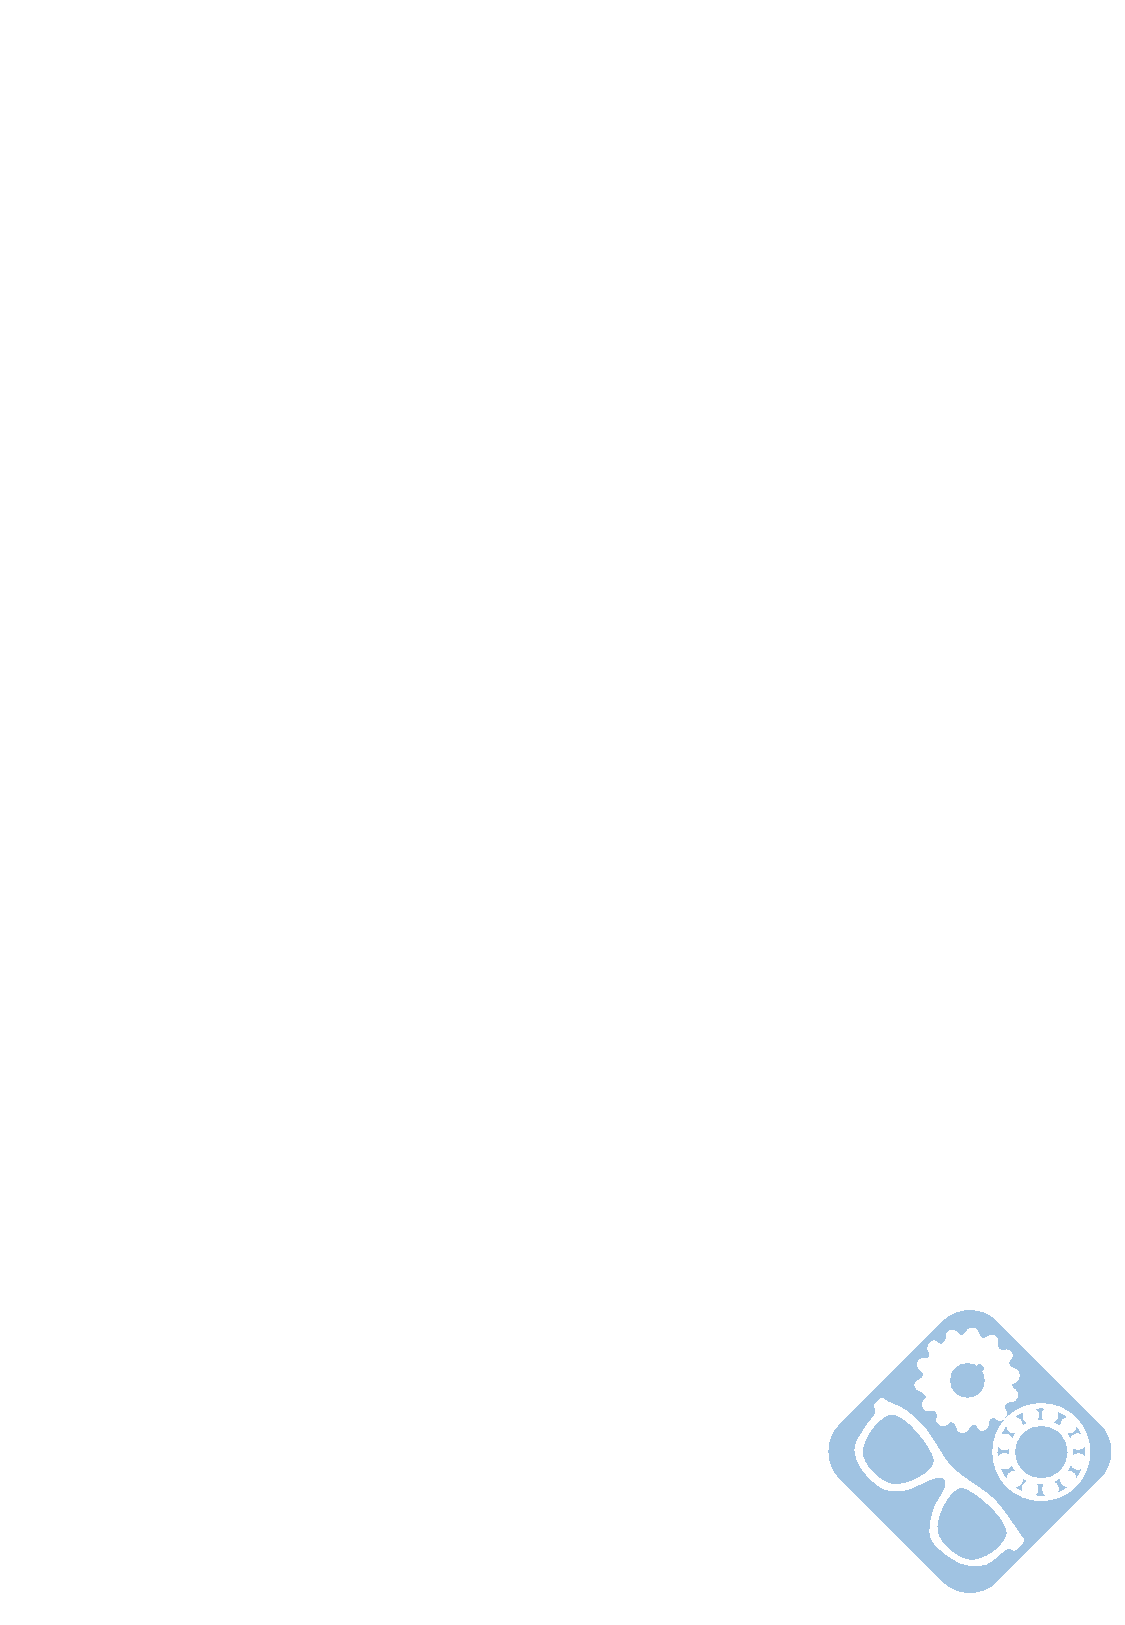
\includegraphics[width=\paperwidth,height=\paperheight,%
keepaspectratio]{../../../img/fond4}%
\end{center}
\vfill
}}}

\begin{document}

\pagestyle{empty}

\AddToShipoutPicture*{\BackgroundPic}


\includegraphics[width=2cm]{../../../img/logo}

\Huge{DS \numero - \sujet}

\vspace{1cm}

\ifdef{\prive}{\begin{center}\colorbox{danger}{\Huge{Avec Correction}}\end{center}}{}

\begin{center}
\centering\huge{PTSI}
\end{center}

\vspace{2cm}


\begin{center}
\centering\Large{\jour}
\end{center}

\vspace{2cm}

\normalsize

\tableofcontents

\newpage

\AddToShipoutPicture{\BackgroundPicdeux}

\pagestyle{fancy}

\begin{center}
\Huge \sujet
\end{center}


\normalsize


\section{Présentation}

Le désherbage des vignes permet de préserver les ressources hydriques et azotées en éliminant les plantes qui entrent en concurrence avec la vigne. Il élimine également les herbes qui montent au cœur du feuillage favorisant
le développement de maladies et contribue à l'aspect esthétique des vignes, vecteur d'image pour le vin.

La zone inter-rang est facile d'accès et l'entretien peut être fait par labour ou par tonte. Le désherbage mécanique « sous le rang » (figure \ref{img01}) est délicat à réaliser, car il faut éviter de heurter les ceps avec l'outil qui travaille la terre.

\begin{figure}[!h]
\centering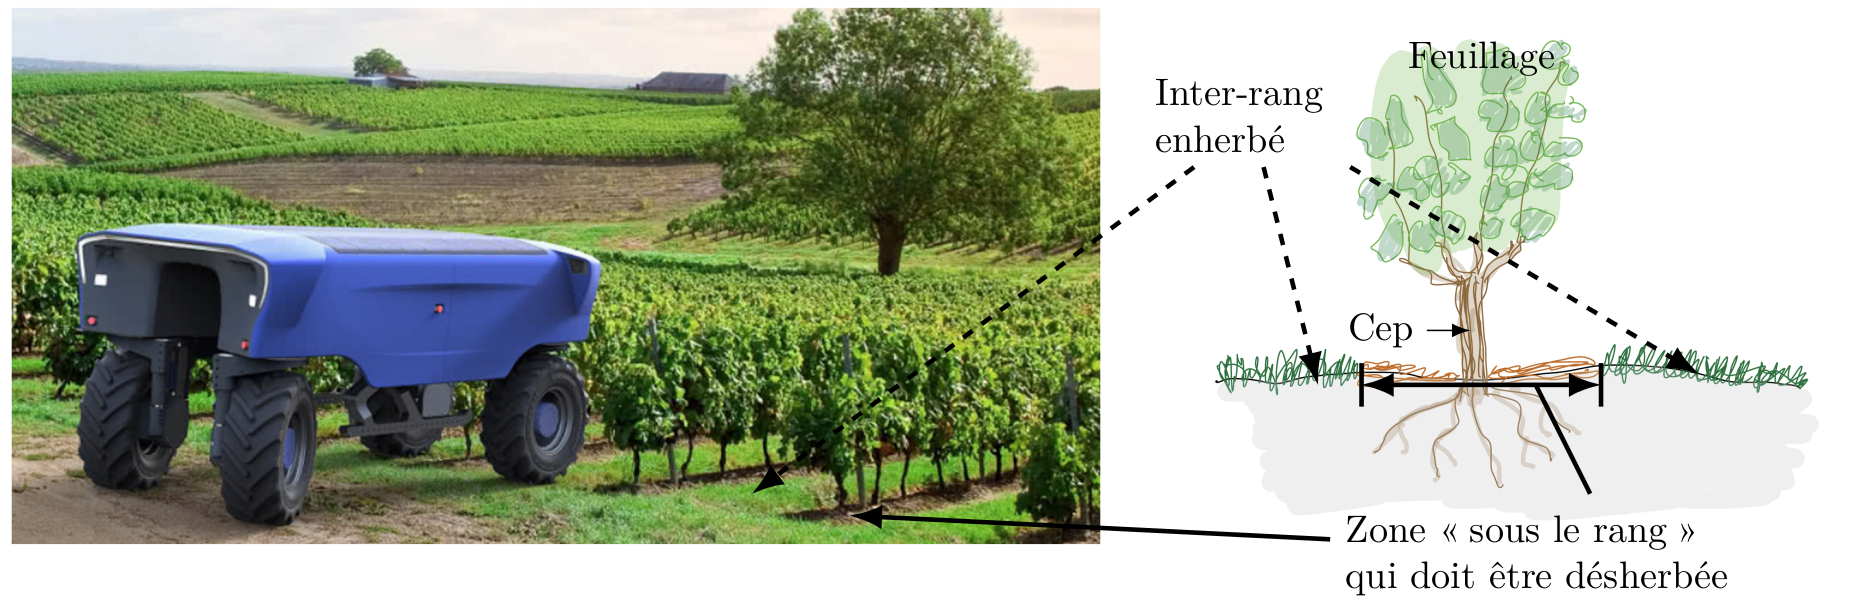
\includegraphics[width=0.8\linewidth]{img/fig01}
 \caption{Robot Bakus (vue de gauche) sans outil dans une vigne avec inter-rang enherbé et espace sous le rang désherbé mécaniquement. Morphologie d'un plan de vigne (vue de droite) et vocabulaire associé}
 \label{img01}
\end{figure}

S'il a l'avantage de décompacter le sol au voisinage des pieds de vigne, ce qui permet de favoriser la circulation de l'air et de l'eau vers le système racinaire des ceps, le désherbage mécanique doit être réalisé dans des conditions d'humidité du sol bien précises afin de garantir la qualité du travail. La conduite des tracteurs nécessite du personnel qualifié et un équipement suffisant pour pouvoir intervenir et traiter l'ensemble du vignoble au moment opportun.

Le désherbage chimique à base d'herbicides, plus facile à mettre \oe uvre et moins onéreux (tableau \ref{table01}), s'est développé au cours des cinquante dernières années malgré les doutes émis sur les substances utilisées vis-à-vis des hommes et de l'environnement.

\begin{table}[ht!]
\begin{center}
\begin{tabular}{|m{5.5cm}|>{\centering\arraybackslash}p{3.5cm}|>{\centering\arraybackslash}p{2.5cm}|>{\centering\arraybackslash}p{3.5cm}|}
\cline{2-4}
\multicolumn{1}{c|}{ }&Désherbage mécanique
\{tracteurs + chauffeurs\} &Désherbage chimique&Désherbage
mécanique robotisé\\
\hline
Coût annuel pour 10 ha de vignes larges (4000 pieds/ha)&300€&130€& à minimiser\\
\hline
Coût annuel pour 10 ha de
vignes étroites (8000 pieds/ha)&800€&180€& à minimiser\\
\hline
Nombre de passages annuels&5&2&5\\
\hline
Émission de gaz à effet de serre
équivalent CO\textsubscript 2 Tank To Wheel&120 kg/an/ha&40 kg/an/ha&à minimiser\\
\hline
\end{tabular}
\end{center}
 \caption{Comparatif des différentes solutions, source Institut Français de la Vigne et du Vin}
 \label{table01}
\end{table}

La robotisation du désherbage mécanique doit devenir la solution utilisée par la majorité des viticulteurs :
\begin{itemize}
 \item en proposant des véhicules capables de suivre le rang de manière autonome afin de s'affranchir des problèmes de disponibilité des chauffeurs et intervenir à tout moment, même la nuit,
 \item en utilisant exclusivement de l'énergie électrique afin de minimiser les émissions de gaz à effet de serre équivalent CO\textsubscript 2 Tank To Wheel (du réservoir à la roue).
\end{itemize}

\begin{figure}[!h]
\begin{minipage}{0.65\linewidth}
L'objet de cette étude est le robot « Bakus » (figure \ref{img01}) de la
société VitiBot dont les premières utilisations ont eu lieu fin 2019 en Champagne. C'est un quadriporteur enjambeur de rang, dont chaque roue est motrice et orientable. L'énergie utilisée est exclusivement électrique, Bakus est équipé de batteries et de panneaux solaires.

~\

Dans ce sujet, seul le cas du désherbage mécanique avec lame décavaillonneuse est étudié car il est le plus exigeant vis-à-vis des
performances attendues du robot. Le décavaillonnage consiste à retourner la terre dans la zone « sous le rang ». Il demande un guidage précis des outils dans le rang de vigne et occasionne une dépense énergétique accrue pour vaincre l'effort du sol sur les lames et assurer le mouvement de retrait de ces dernières à l'approche d'un cep afin d'éviter de l'abimer.

Les ceps de vigne sont plantés à des intervalles interceps réguliers de longueur $l_{ic},$ tels que $1m\leq l_{ic}\leq 1.2m$, pour former le rang.

Le cahier des charges partiel du désherbage mécanique des vignes
est donné figure \ref{img03}.
\end{minipage}\hfill
\begin{minipage}{0.3\linewidth}
\centering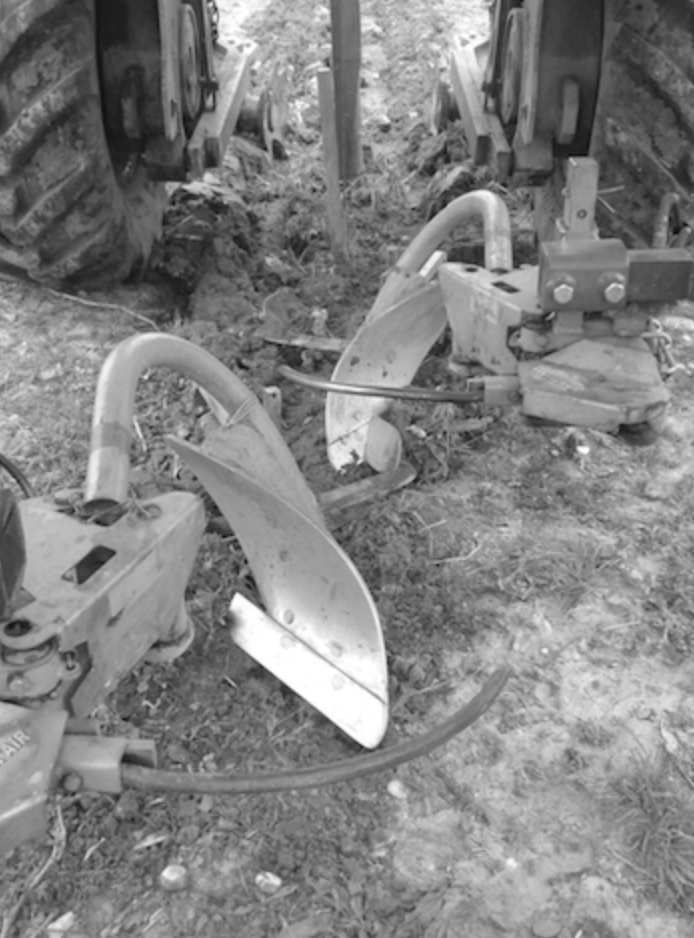
\includegraphics[width=0.95\linewidth]{img/fig02}
 \caption{Lames décavaillonneuses interceps équipant un enjambeur}
 \label{img02}
\end{minipage}
\end{figure}

\begin{figure}[!h]
\centering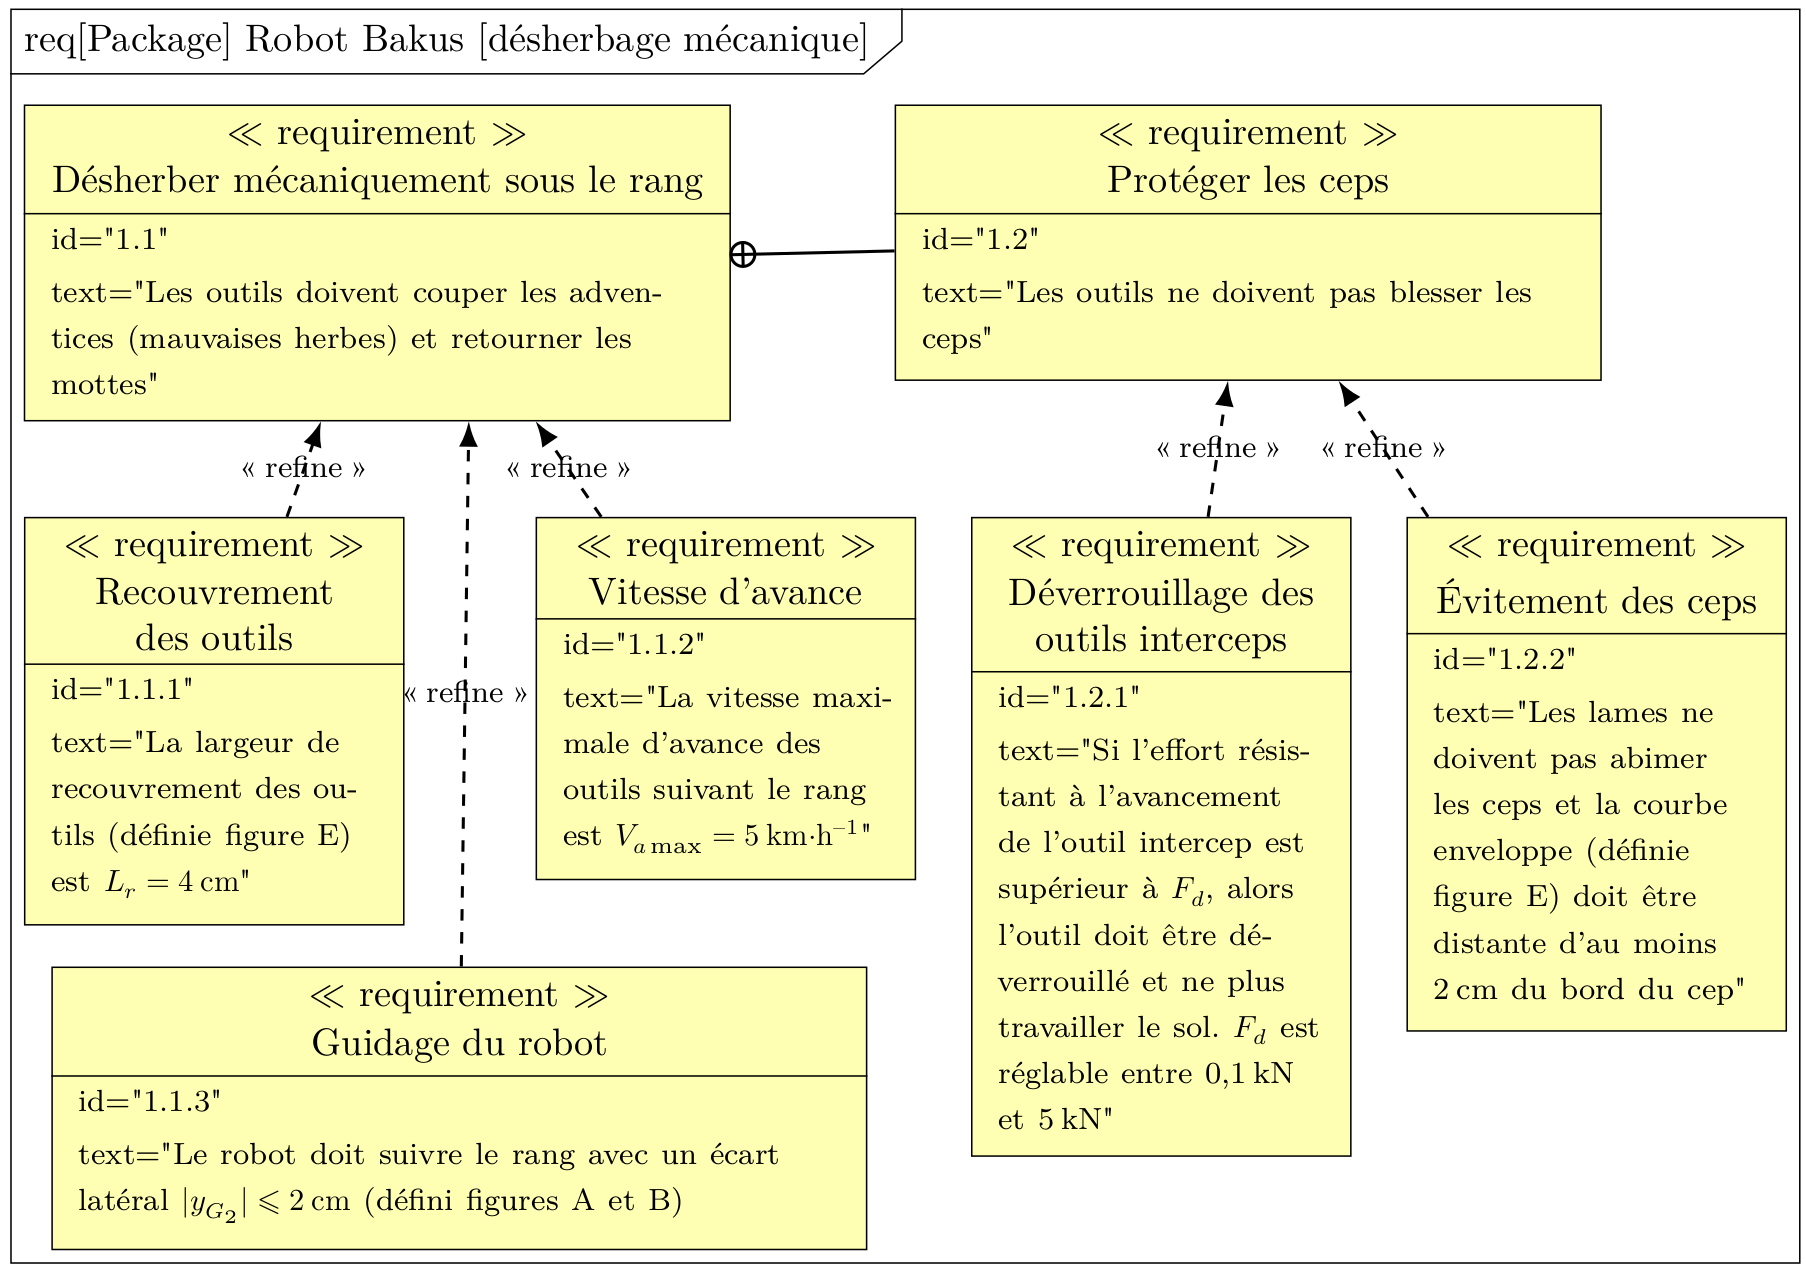
\includegraphics[width=0.8\linewidth]{img/fig03}
 \caption{Cahier des charges partiel}
 \label{img03}
\end{figure}

L'objet de ce sujet est d'évaluer les solutions retenues pour suivre le rang de manière autonome et assurer le retrait des lames décavaillonneuses à l'aide d'un actionneur électrique tout en optimisant la consommation énergétique et en respectant les exigences du désherbage mécanique.

Le sujet est décomposé en deux parties :
\begin{itemize}
\item en partie II, il s'agit d'élaborer la consigne de guidage du robot Bakus le long du rang à partir des informations issues des capteurs utilisés et de vérifier les performances du guidage vis-à-vis du désherbage mécanique dans le cas de sols glissants en dévers,
 \item en partie III, une étude du mécanisme de retrait d'une lame décavaillonneuse permettra d'estimer la puissance économisée lors de l'évitement d'un cep, puis une étude dynamique permettra de choisir un actionneur électrique et de concevoir une stratégie de commande de ce dernier.
\end{itemize}

\section{Génération des consignes d'orientation des roues avant et arrière
pour le guidage du robot Bakus}

\paragraph{Objectif}

Élaborer les lois permettant de générer les consignes d'orientation à envoyer à chacune des quatre roues orientables du robot, afin qu'il puisse se déplacer le long d'un rang de vigne avec la même précision qu'un tracteur piloté par un chauffeur.

Pour que le robot puisse se déplacer correctement le long du rang qu'il enjambe, il faut qu'il puisse suivre la trajectoire $\mathcal{T}$ le plus précisément possible.

Afin de simplifier l'étude proposée, il sera supposé dans toute cette partie que la trajectoire $\mathcal{T}$ à suivre par le robot, correspondant à la courbe passant par l'ensemble des ceps de vigne d'un rang, est une droite $(O,\vec{x}_0)$ (figure \ref{annexeA}). En effet, les rangs de vignes sont globalement plantés en ligne droite (ou avec des rayons de courbure très grands devant la distance entre deux ceps successifs) et avec une erreur de positionnement de quelques millimètres, très inférieure aux dimensions du robot.

Les différents outils que le robot embarque travaillant au milieu du robot (point $G_2$), ce dernier doit piloter les angles d'orientation de ses roues avant et arrière, afin de maîtriser l'écart latéral $y_{G_2}$ et l'écart angulaire $\theta$ (compensation de la marche en crabe sur les terrains en pente glissants, voir figure \ref{annexeA}).

\subsection{Changement de variables ($y_{G_2}$,$\theta$) $\rightarrow$ ($y_F$ , $y_R$)}

\paragraph{Objectif}

Simplifier l'approche du problème d'asservissement du couple de variables ($y_{G_2}$,$\theta$) au point de fonctionnement ($0$,$0$) à l'aide d'un changement de variables approprié.

L'écart angulaire $\theta$ (figures \ref{annexeA}) n'est en réalité que de quelques degrés ($|\theta|\leq 7$\textdegree).

Ainsi, à l'ordre 1, il est possible d'utiliser dans la suite les approximations suivantes :
$cos \theta \approx 1$,
$sin \theta \approx \theta$
et $tan \theta \approx \theta$.

\question{Écrire les vecteurs $\overrightarrow{G_0F_0}$, $\overrightarrow{F_0F}$, $\overrightarrow{FG_2}$, $\overrightarrow{G_2G_0}$, respectivement dans les bases $\mathcal{B}_0$, $\mathcal{B}_0$, $\mathcal{B}_2$ et $\mathcal{B}_0$.}

\question{Faire une figure de changement de repère et écrire tous les vecteurs unitaires de la base $\mathcal{B}_2$ dans la base $\mathcal{B}_0$.}

\question{Projeter les vecteurs de la question 1 dans la base $\mathcal{B}_0$.}

\question{Développer une fermeture vectorielle à partir des vecteurs de la question 1. En déduire une expression de $y_F$ en fonction de $y_{G_2}$, $\theta$ et $L$}

\question{Écrire les vecteurs $\overrightarrow{R_0G_0}$, $\overrightarrow{G_0G_2}$, $\overrightarrow{G_2R}$, $\overrightarrow{RR_0}$, respectivement dans les bases $\mathcal{B}_0$, $\mathcal{B}_0$, $\mathcal{B}_2$ et $\mathcal{B}_0$.}

\question{Projeter ces vecteurs dans la base $\mathcal{B}_0$.}

\question{Développer une fermeture vectorielle à partir des vecteurs de la question 5. En déduire une expression de $y_R$ en fonction de $y_{G_2}$, $\theta$ et $L$}

\question{Linéariser les expressions des questions 4 et 7 grâce aux approximations d'ordre 1.}

\question{En déduire l'expression de $\theta$ en fonction de $y_F$, $y_R$ et $L$.}

\subsection{Modélisation cinématique étendue du robot}

\paragraph{Objectif}

Établir un modèle exploitable décrivant les déplacements du robot Bakus sur un sol naturel, c'est-à-dire en tenant compte d'un éventuel glissement des roues sur le sol lorsqu'il est en dévers (phénomène de dérive latérale et angulaire).

Pour pouvoir élaborer les consignes d'orientation des roues du robot, il est nécessaire d'établir un modèle reflétant avec précision le comportement réel du système. Un modèle dynamique complet serait idéal, mais sa complexité rendrait difficile toute étude de loi de commande, notamment à cause de nombreux paramètres difficiles à estimer.

À contrario, un modèle cinématique sous hypothèse de roulement pur sans glissement au niveau du contact roue-sol serait plus facile à gérer d'un point de vue de l'élaboration de la commande qu'un modèle dynamique complet, mais il ne décrirait pas suffisamment bien le comportement du système réel qui peut rencontrer des problèmes d'adhérence sur un sol naturel en dévers.

\begin{figure}[!h]
\centering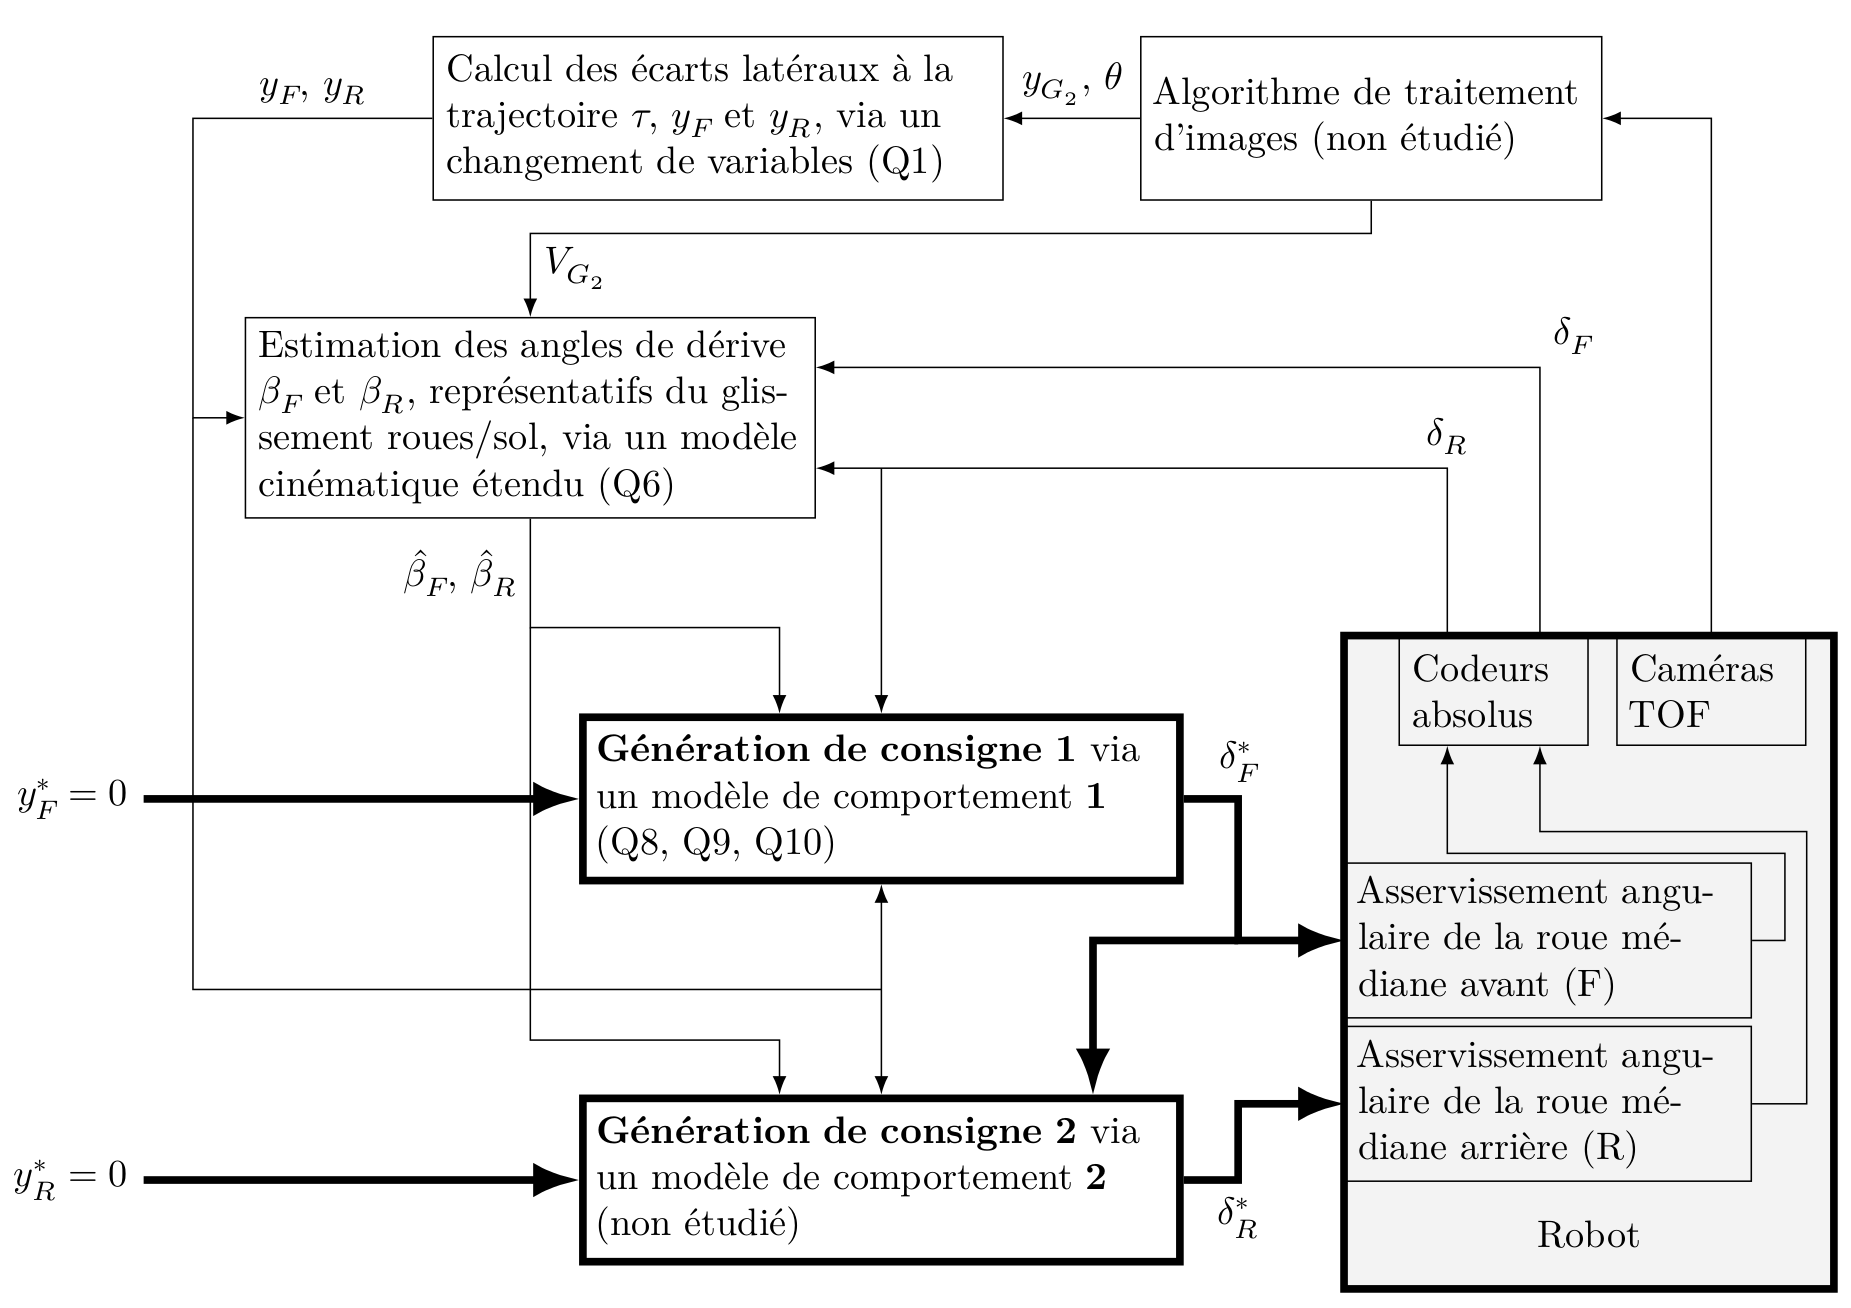
\includegraphics[width=0.8\linewidth]{img/fig04}
 \caption{Schéma de principe de la génération des consignes d'orientation des roues du robot Bakus $\delta^*_F$ et $\delta^*_R$ pour le suivi de la trajectoire $\mathcal{T}$, avec prise en compte du glissement au niveau des roues sur le sol ($Qi$ fait référence au(x) résultat(s) de la question i), $y^*_F$ et $y^*_R$ correspondent aux écarts latéraux souhaités entre le robot et la trajectoire $\tau$ (figure \ref{annexeA}).}
 \label{img04}
\end{figure}

Une approche intermédiaire consiste alors à enrichir le modèle cinématique du robot Bakus avec un nombre limité de variables dynamiques. C'est cette approche qui est retenue par la suite, en ajoutant des variables
de glissement sur chacun de ses trains directeurs et roulants. Ce modèle, dit modèle cinématique étendu, est représenté sur la figure \ref{annexeA}.

\subsubsection{Notations et hypothèses}

Les notations suivantes sont relatives à la figure \ref{annexeA}.
\begin{itemize}
 \item le sol est modélisé par le solide $0$ auquel est associé le repère $(O,\vec{x}_0,\vec{y}_0,\vec{z}_0)$ et est supposé être localement plan à l'aplomb du point G 2,
 \item le problème est considéré comme cinématiquement plan dans $(O,\vec{x}_0,\vec{y}_0,\vec{z}_0)$,
 \item le châssis du robot Bakus correspond au solide 2, associé au repère $(G_2,\vec{x}_2,\vec{y}_2,\vec{z}_2)$,
 \item afin de simplifier l'étude, les deux roues avant sont assimilées à une seule roue virtuelle (repère 5) située en $F$, de même le train arrière est assimilé à une roue virtuelle (repère 6) située en $R$ (figure \ref{annexeA}),
 \item les angles $\delta_F=(\vec{x}_2,\vec{x}_F)$ et $\delta_R=(\vec{x}_2,\vec{x}_R)$ sont respectivement les angles d'orientation autour de $\vec{z}_2$ de la roue virtuelle avant en $F$ et de la roue virtuelle arrière en $R$. Ces deux angles constituent les deux premières variables de commande du robot. $V_{G_2}$ est la mesure algébrique de la vitesse linéaire du robot au point $G_2$ et correspond à la troisième variable de commande ;
 \item les angles $\beta_F=(\vec{x}_{V_F},\vec{x}_F)$ et $\beta_R=(\vec{x}_{V_R},\vec{x}_R)$ sont respectivement les angles de dérive des roues virtuelles avant et arrière. Ces angles traduisent la conséquence d'un glissement éventuel des roues virtuelles avant et arrière par rapport au sol,
 \item l'angle $\theta$ est défini par $\theta=(\vec{x}_0,\vec{x}_2)$. Il paramètre l'orientation du châssis 2 du robot par rapport à la
trajectoire T,
 \item la dérivée temporelle d'une variable $s$ sera notée $\dot{s}=\frac{ds}{dt}$,
 \item quel que soit le point $P\in\left\{F,G_2,R\right\}$:
 \begin{itemize}
  \item $\overrightarrow{OP}=x_P\cdot\vec{x}_0-y_P\cdot\vec{y}_0$,
  \item $\vec{V}_{P,2/0}=\vec{V}_P$ correspond au vecteur vitesse réel, c'est-à-dire malgré le glissement des roues sur le sol, du point P pris dans le mouvement du châssis 2 du robot par rapport au sol. Ainsi, il vient $\dot{x}_P=\vec{V}_P\cdot\vec{x}_0$ et $\dot{y}_P=\vec{V}_P\cdot\vec{y}_0$,
  \item les angles $\gamma_P$ sont définis par $\gamma_P=(\vec{x}_2,\vec{x}_{V_P})$,
  \item $P_0$ correspond au projeté orthogonal d'un point $P$ lié au robot sur $\mathcal{T}$,
  \item $I_{20}$ correspond à un point virtuel tel que $\vec{V}_{I_{20},2/0}=\vec{0}$. Il est alors possible de montrer que $\vec{V}_P\cdot\overrightarrow{I_{20}P}=\vec{0}$,
  \item la vitesse linéaire d'avance du robot le long de la trajectoire $\mathcal{T}$ correspond à $\vec{x}_{G_2}$.
 \end{itemize}
\end{itemize}

Les valeurs des variables $\theta$ (en radian) et $y_{G_2}$ (en mètre) sont déterminées par le robot grâce à un algorithme de traitement d'images de huit caméras TOF (Time Of Flight) installées sur la périphérie du robot.

\subsubsection{Mise en équation du modèle cinématique étendu du robot Bakus}

\question{Après avoir justifié que $\vec{V}_{F,2/0}=\left[\frac{d\overrightarrow{OF}}{dt}\right]_{R0}$ et $\vec{V}_{R,2/0}=\left[\frac{d\overrightarrow{OR}}{dt}\right]_{R0}$, déterminer $\vec{V}_{F,2/0}$ et $\vec{V}_{R,2/0}$, en fonction de $\dot{x}_F$, $\dot{y}_F$, $\dot{x}_R$ et $\dot{y}_R$ dans la base $\mathcal{B}_0$.}

\question{Faire les figures de changement de repère et écrire tous les vecteurs unitaires des bases $\mathcal{B}_{V_F}$ et $\mathcal{B}_{V_R}$ dans la base $\mathcal{B}_0$.}

\question{En déduire $\vec{V}_{F,2/0}$ et $\vec{V}_{R,2/0}$, en fonction de $V_F$, $V_R$ dans la base $\mathcal{B}_0$.}

\question{En déduire les relations donnant les expressions de $\dot{y}_F$ et $\dot{y}_R$ en fonction de $V_F$, $V_R$, $\theta$, $\delta_F$, $\delta_R$, $\beta_F$ et $\beta_R$.}

\question{En utilisant la même méthode (que questions 10, 11, 12 et 13), déterminer les relations donnant l'expression de $\dot{x}_{G_2}$ en fonction de $V_{G_2}$, $\gamma_{G_2}$ et $\theta$.}

\question{Déterminer la relation entre $\vec{V}_{G_2,2/0}$, $\vec{V}_{F,2/0}$, $\overrightarrow{G_2F}$ et $\vec{\Omega}_{2/0}$}

\question{Montrer que $\left(\overrightarrow{G_2F}\wedge\vec{\Omega}_{2/0}\right)\cdot\vec{x}_2=0$}

\question{En déduire que $\vec{V}_{G_2}\cdot\vec{x}_2=\vec{V}_{F}\cdot\vec{x}_2=\vec{V}_{R}\cdot\vec{x}_2$}

\question{En déduire une relation entre $V_{G_2}$, $\gamma_{G_2}$, $V_F$, $\gamma_F$, $V_R$ et $\gamma_R$.}

\question{A partir des résultats aux questions 13, 14, 18 et des hypothèses concernant les approximations à l'ordre 1, montrer que:\\
$\left \{
\begin{array}{rcl}
\dot{x}_{G_2}&=&V_{G_2}\\
\dot{y}_F&=&-V_{G_2}\cdot (\theta+\delta_F-\beta_F)\\
\dot{y}_R&=&-V_{G_2}\cdot (\theta+\delta_R-\beta_R)
\end{array}
\right.$}

\subsection{Mesure ou estimation des variables du modèle cinématique étendu}

\paragraph{Objectif}

Donner les moyens au robot de mesurer ou, à défaut, d'estimer les valeurs des variables $\delta_F$, $\delta_R$, $y_{G_2}$, $\theta$, $\dot{y}_F$, $\dot{y}_R$ et $V_{G_2}$ du modèle cinématique étendu.

\subsubsection{Variables mesurées directement par des capteurs dédiés}

\paragraph{Mesure de l'orientation des roues}

L'orientation des roues, paramétrée par les variables $\delta_F$ et $\delta_R$, est effectuée par des motoréducteurs asservis en position. La mesure de $\delta_F$ et $\delta_R$ est effectuée par l'intermédiaire de codeurs angulaires absolus situés en sortie de réducteur.

\question{Quelle est la différence entre des codeurs angulaires absolus et des codeurs relatifs (incrémentaux).}

\paragraph{Mesure des variables cinématiques}

L'analyse des images successives prises par les caméras TOF permet au robot de déterminer les valeurs des variables $y_{G_2}$, $\theta$ et $V_{G_2}$. 

Ce traitement n'est pas étudié dans ce sujet.

L'évaluation des variables:
\begin{itemize}
  \item $y_F$ et $y_R$ se fait à l'aide des valeurs de $y_{G_2}$, $\theta$ et des relations de changement de variables trouvés précédemment,
  \item $\dot{y}_F$, $\dot{y}_R$ se fait à partir de la dérivation temporelle des variables $y_F$ et $y_R$.
\end{itemize}

\subsubsection{Variables estimées par analyse d'images des huit caméras TOF du robot}

Le problème majeur pour la commande du robot Bakus est qu'il est très difficile de mesurer les valeurs des variables de glissement $\beta_F$ et $\beta_R$ à l'aide de capteurs dédiés. L'idée consiste à estimer ces variables de glissement, notées alors $\widehat{\beta}_F$ et $\widehat{\beta}_R$, à partir des autres grandeurs mesurées par le système.

\question{À partir des équations de la question 19, donner l'expression des variables estimées $\widehat{\beta}_F$ et $\widehat{\beta}_R$ en fonction
des variables mesurées $\dot{y}_F$, $\dot{y}_R$, $V_{G_2}$, $\theta$, $\delta_F$ et $\delta_R$.}

Grâce au modèle cinématique étendu établi précédemment, les variables de glissement estimées $\widehat{\beta}_F$ et $\widehat{\beta}_R$ peuvent
donc être déterminées par le robot, à partir des mesures fournies par les codeurs absolus des dispositifs d'orientation des roues et l'analyse des images acquises par les huit caméras TOF.

On trouve sur le document réponse le tracé de $\dot{y}_F$, $V_{G_2}$, $\theta$, $\delta_F$. 

\question{Compléter le tableau du document réponse avec les valeurs numériques lues sur la courbe, déterminer $\widehat{\beta}_F$ à partir de la formule précédente et tracer la courbe de $\widehat{\beta}_F$.}

\question{Justifier que l'hypothèse présentée juste avant la question 1 peut être utilisée dans ce contexte.}

\section{Optimisation énergétique du mouvement de retrait d'une lame
décavaillonneuse, choix d'un actionneur et conception de sa com-
mande}

Le robot Bakus étant capable de suivre le rang de manière autonome, il est nécessaire d'étudier le mécanisme qui permet à la lame décavaillonneuse d'éviter les ceps. Ce mouvement de retrait devant le cep consomme de l'énergie, mais il est possible de diminuer l'effort résistant à l'avancement du robot lors du retrait en utilisant un système de transformation de mouvement particulier. De plus, il est nécessaire de choisir un actionneur électrique permettant de fournir une dynamique adaptée à l'évitement des ceps, quelles que soient les conditions d'utilisation.

\paragraph{Objectif}

Adapter un outil intercep non motorisé utilisé avec les tracteurs traditionnels afin de concevoir un outil avec motorisation électrique pour le robot Bakus.

\begin{figure}[!h]
\centering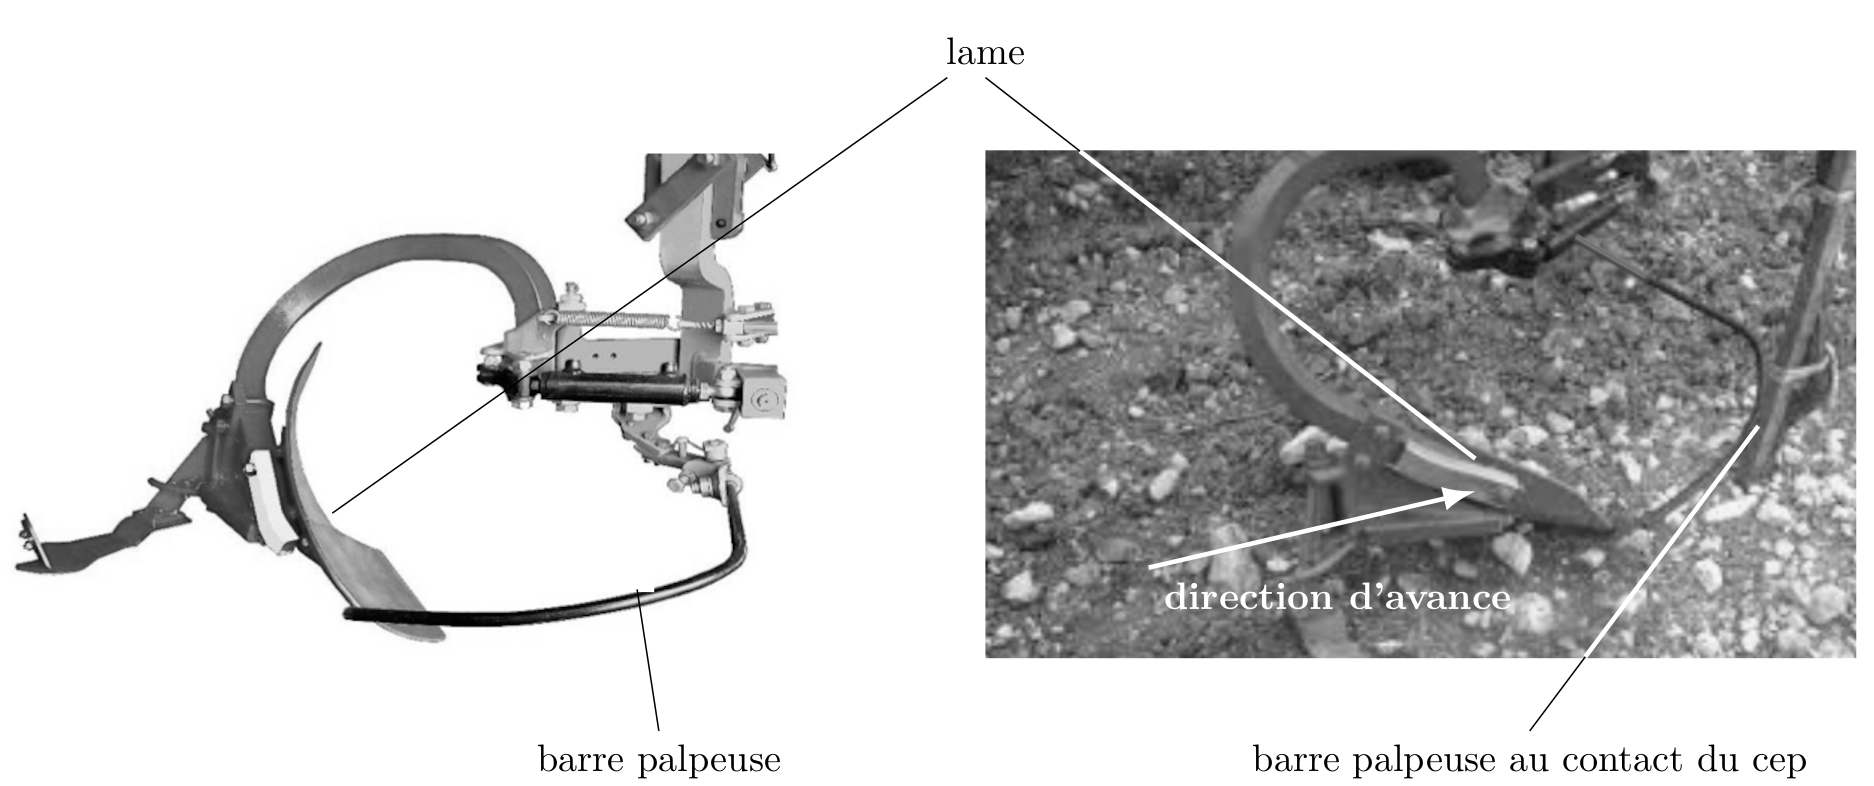
\includegraphics[width=0.8\linewidth]{img/fig05}
 \caption{Vues d'un outil intercep non motorisé en travail (photo de droite), lame et barre palpeuse}
 \label{img05}
\end{figure}

Au contact du cep, une barre palpeuse (figure \ref{img05}) est mise en rotation par rapport au robot. La mise en rotation est d'autant plus rapide que le robot avance vite ou que le cep est proche de l'axe de rotation de la barre palpeuse. Les outils non motorisés utilisent l'action du cep sur la barre palpeuse pour réaliser le mouvement de
retrait, ce qui peut abimer le cep. Les outils motorisés utilisent la barre palpeuse comme un capteur qui permet d'élaborer la commande de l'actionneur qui génère le mouvement de retrait.

\subsection{Modélisation du mouvement des lames, tracé numérique des relations entre paramètres géométriques d'entrée et de sortie puis estimation de la puissance épargnée}

Diminuer la largeur de terre travaillée (notée $Lt$ sur la figure \ref{annexeE} du document réponse) permet de diminuer l'effort résistant à l'avancement du sol sur la lame, et donc de réduire la puissance nécessaire à faire avancer le robot le long du rang. Ce gain de puissance peut alors être affecté au mécanisme de retrait dont la puissance initialement allouée est limitée à 20 kW.

\paragraph{Objectif}

Choisir un mécanisme de transformation du mouvement qui permette de diminuer d'au moins 15 \% la puissance de cette action mécanique lorsque l'outil est en position moyenne de retrait par rapport
à la position déployée : $\Delta\% P sol\rightarrow 4/0 > 15 \%$.
La majorité des outils interceps utilise un mécanisme qui permet de faire reculer la lame, partie de l'outil qui
travaille le sol (figure \ref{img05}), perpendiculairement à la direction d'avance du tracteur afin de ne pas endommager le
cep.

\subsection{Écriture de la loi entrée/sortie géométrique}

La base $\mathcal{B}^*_4=(\vec{u}_4,\vec{v}_4,\vec{z}_0)$ est aussi associée au solide 4 et l'angle entre $\vec{x}_4$ et $\vec{u}_4$ est noté $\alpha_4=(\vec{x}_4,\vec{u}_4)=0.65rad$. La base $\mathcal{B}_3=(\vec{x}_3,\vec{y}_3,\vec{z}_0)$ est associée au solide 3 et l'angle entre $\vec{x}_3$ et $\vec{x}_2$ est noté $\theta_{30}=(\vec{x}_2,\vec{x}_3)=(\vec{y}_2,\vec{y}_3)$.

Les vecteurs suivants sont donnés :
\begin{itemize}
 \item $\overrightarrow{O_1A}=-l_1\cdot\vec{x}_1$,
 \item $\overrightarrow{AB}=-l_4\cdot\vec{y}_4$,
 \item $\overrightarrow{BO_3}=l_3\cdot\vec{x}_3$,
 \item $\overrightarrow{O_3O_1}=-a\cdot\vec{x}_2+b\cdot\vec{y}_2$.
\end{itemize}

Le mouvement de l'intercep permet de passer de la position déployée ($\theta_{10}=0.87rad$) à la position de retrait qui fluctue en fonction de la morphologie de la vigne :
\begin{itemize}
 \item la position de retrait maximale est obtenue pour un angle 
$\theta_{10}=0.1 rad$ (recul du point D de la lame de 18 cm suivant $\vec{y}_0$, voir figure \ref{annexeE}),
 \item la position de retrait moyenne au cours du désherbage d'un rang correspond à une valeur d'angle voisine de $0.3rad$ pour $\theta_{10}$.
\end{itemize}

\question{Écrire sous forme vectorielle la relation de fermeture de la chaîne géométrique liée au modèle de la figure \ref{annexeE} et donner les équations scalaires associées en projection sur les vecteurs de la base $\mathcal{B}_2$.}

\question{En exprimant les fonctions $f_1$, $f_2$ et $f_3$ en fonction des paramètres $l_1$, $l_3$, $l_4$, $a$, $b$, $cos(\theta_{10})$ et $sin(\theta_{10})$, montrer qu'il est possible d'obtenir à partir des équations de la question précédente une seule équation de la
forme :}

\begin{center}
$f_1(\theta_{10})-f_2(\theta_{10})\cdot	sin(\theta_{40})-f_3(\theta_{10}) \cdot cos(\theta_{40})=0$
\end{center}

\section{Implantation l'actionneur}

On propose de motoriser l'intercep à l'aide d'un actionneur, qui est un vérin linéaire électrique

\subsection{Commande de l'actionneur}

\paragraph{Objectif}

Valider le pilotage séquentiel de l'actionneur et choisir un correcteur pour la boucle de vitesse vis-à-vis des exigences du désherbage mécanique.

On donne dans le document réponse le schéma bloc de l'asservissement de cet actionneur. Dans ce modèle, on retrouve un correcteur dont la fonction de transfert est $C(p)=K_c$ et le vérin électrique, modélisé par un
gain pur $K_{verin}$.

On précise que :
\begin{itemize}
 \item l'erreur est définie par $\varepsilon(p)=\dot{\lambda}_{cons}-\dot{\lambda}$,
 \item l'équation de la résultante du Principe Fondamental de la Dynamique appliqué au vérin:\\
  $M_{eq}\cdot \frac{d\dot{\lambda}(t)}{dt}=F_{mot}-F_{sol}\cdot k_{p\ MAX}$
\end{itemize}

\question{Compléter le schéma bloc à partir des informations disponibles dans le sujet et de vos connaissances.}

\question{Déterminer les fonctions de transfert $H_1(p)$ et $H_2(p)$ qui permettent d'écrire $\dot{\lambda}$ de la manière suivante:

\begin{center}
$\dot{\lambda}=H_1(p)\cdot \dot{\lambda}_{cons}+H_2(p)\cdot \left(-F_{sol}\cdot k_{p\ MAX}\right)$
\end{center}

Les mettre sous la forme canonique et déterminer leurs ordres et classes.}

\question{Déterminer l'unité de $\frac{M_{eq}}{K_c\cdot K_{verin}}$ ? Était-ce prévisible ?}

Pour la suite, on prendra $H_2(p)=\frac{6\cdot10^{-5}\cdot p}{1+6\cdot10^{-5}\cdot p}$

\question{Tracer le diagramme de Bode de $H_2(p)$.}

\section{Modélisation volumique}

\question{Compléter les vues du document réponse.}

\newpage

\section{Annexes}

\begin{figure}[!h]
\centering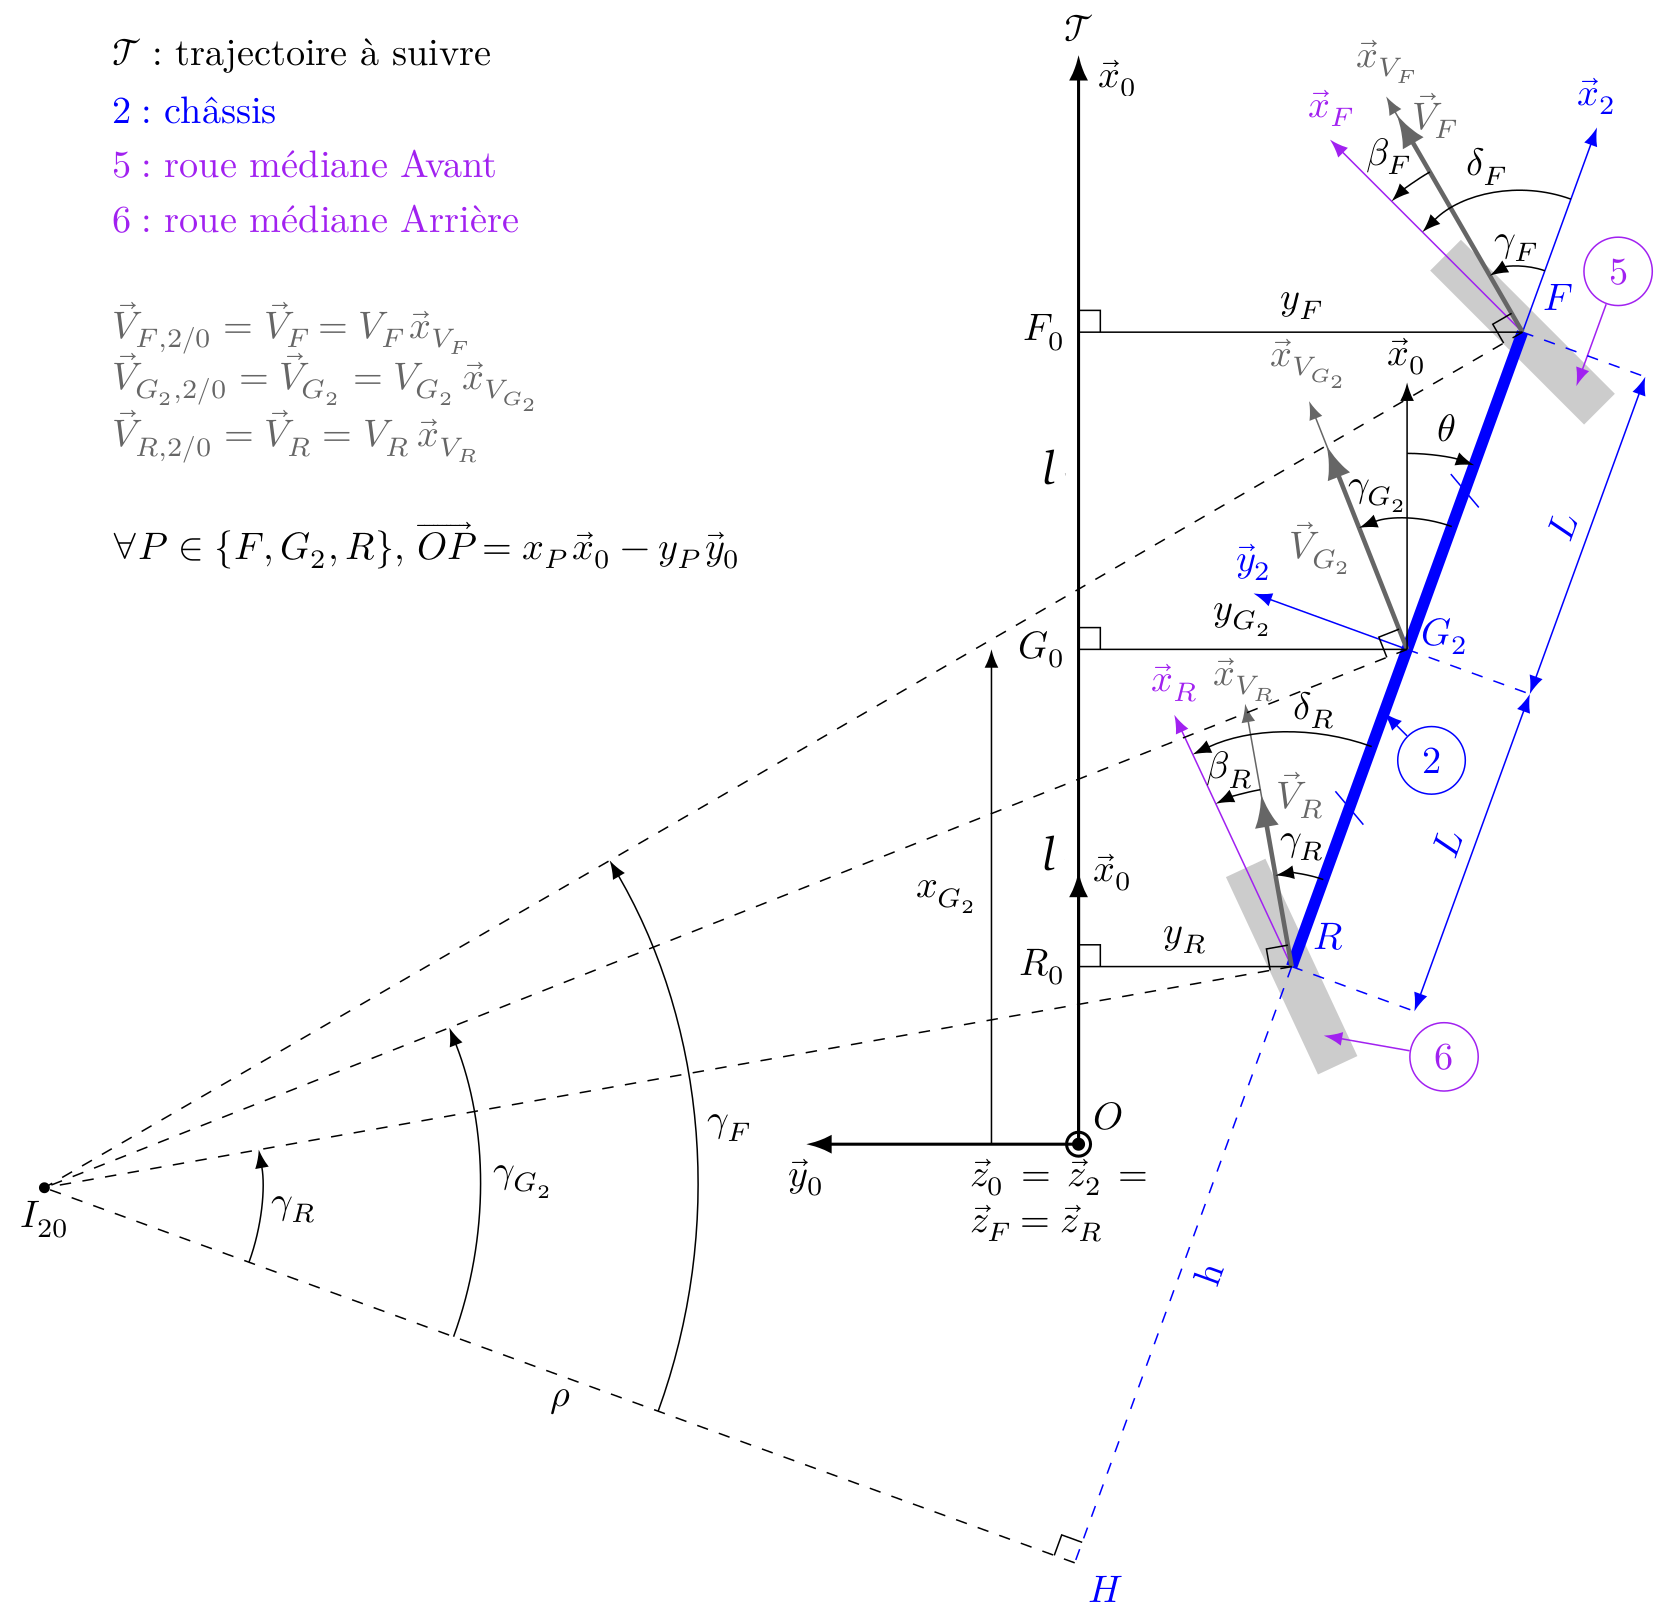
\includegraphics[width=0.85\linewidth]{img/figA.png} \caption{Vue de dessus d'un modèle cinématique étendu de type « bicyclette » dans le cas d'une trajectoire rectiligne T à suivre par le robot (configuration pour laquelle $\theta < 0$). Les roues médianes 5 et 6 peuvent être orientées en pivotant respectivement autour de $(F,\vec{z}_F) = (F,\vec{z}_2)$ et $(R,\vec{z}_F) = (R,\vec{z}_2)$}
 \label{annexeA}
\end{figure}

\newpage

\begin{figure}[!h]
\centering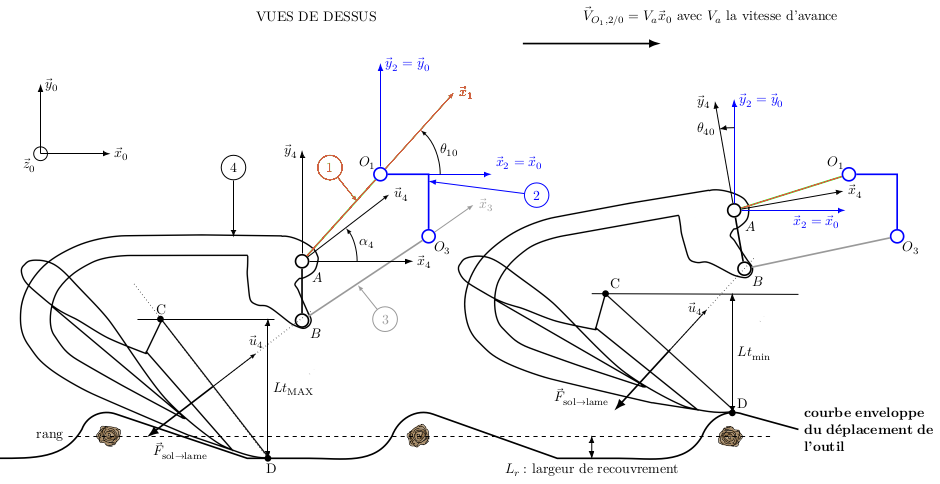
\includegraphics[width=1.3\linewidth,angle=90]{img/figE.png} \caption{Modélisation de l'outil intercep et de sa lame en position déployée (à gauche) et en position de retrait (à droite) en vue de dessus (barre palpeuse non représentée).}
 \label{annexeE}
\end{figure}

\cleardoublepage

\ifdef{\public}{\pagestyle{documentreponse}}{\pagestyle{correction}}

\reponse{5}{}{
$\left \{
\begin{array}{rcl}
\overrightarrow{G_0F_0}&=&l\cdot \vec{x}_0\\
\overrightarrow{F_0F}&=&-y_F\cdot \vec{y}_0\\
\overrightarrow{FG_2}&=&-L\cdot \vec{x}_2\\
\overrightarrow{G_2G_0}&=&y_{G_2}\cdot \vec{y}_0
\end{array}
\right.$
}

\reponse{4}{}{
\begin{minipage}{0.6\linewidth}
$\left \{
\begin{array}{rcl}
\vec{x}_2&=&cos\theta\cdot\vec{x}_0+sin\theta\cdot\vec{y}_0\\
\vec{y}_2&=&-sin\theta\cdot\vec{x}_0+cos\theta\cdot\vec{y}_0\\
\vec{z}_2&=&\vec{z}_0\\
\end{array}
\right.$
\end{minipage}\hfill
\begin{minipage}{0.35\linewidth}
\centering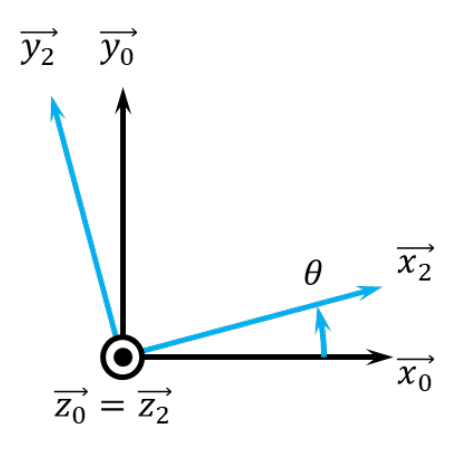
\includegraphics[width=0.6\linewidth]{img/figcor1}
\end{minipage}
}

\reponse{3}{}{
$\left \{
\begin{array}{rcl}
\overrightarrow{G_0F_0}&=&l\cdot \vec{x}_0\\
\overrightarrow{F_0F}&=&-y_F\cdot \vec{y}_0\\
\overrightarrow{FG_2}&=&-L\cdot(cos\theta\cdot\vec{x}_0+sin\theta\cdot\vec{y}_0)\\
\overrightarrow{G_2G_0}&=&y_{G_2}\cdot \vec{y}_0
\end{array}
\right.$
}

\reponse{4}{}{
$\overrightarrow{G_0F_0}+\overrightarrow{F_0F}+\overrightarrow{FG_2}+
\overrightarrow{G_2G_0}=\vec{0}$

$-y_F-L\cdot sin\theta+y_{G_2}=0$
}
\ifdef{\public}{\newpage}


\reponse{3}{}{
$\left \{
\begin{array}{rcl}
\overrightarrow{R_0G_0}&=&l\cdot \vec{x}_0\\
\overrightarrow{G_0G_2}&=&-y_{G_2}\cdot \vec{y}_0\\
\overrightarrow{G_2R}&=&-L\cdot \vec{x}_2\\
\overrightarrow{RR_0}&=&y_R\cdot \vec{y}_0
\end{array}
\right.$
}

\reponse{3}{}{
$\left \{
\begin{array}{rcl}
\overrightarrow{R_0G_0}&=&l\cdot \vec{x}_0\\
\overrightarrow{G_0G_2}&=&-y_{G_2}\cdot \vec{y}_0\\
\overrightarrow{G_2R}&=&-L\cdot(cos\theta\cdot\vec{x}_0+sin\theta\cdot\vec{y}_0)\\
\overrightarrow{RR_0}&=&y_R\cdot \vec{y}_0
\end{array}
\right.$
}

\reponse{3}{}{
$\overrightarrow{R_0G_0}+\overrightarrow{G_0G_2}+\overrightarrow{G_2R}+\overrightarrow{RR_0}=\vec{0}$

$-y_{G_2}-L\cdot sin\theta+y_R=0$
}

\reponse{2}{}{
$\left \{
\begin{array}{rcl}
-y_F-L\cdot \theta+y_{G_2}=0\\
-y_{G_2}-L\cdot \theta+y_R=0
\end{array}
\right.$
}

\reponse{2}{}{
$-y_F-L\cdot \theta-L\cdot \theta+y_R=0$

Donc, $\theta=\frac{y_R-y_F}{2\cdot L}$
}

\ifdef{\public}{\newpage}

\reponse{4}{}{
$\left \{
\begin{array}{rcl}
\vec{V}_{F,2/0}=\dot{x}_F\cdot \vec{x}_0-\dot{y}_F\cdot \vec{y}_0 \\
\vec{V}_{R,2/0}=\dot{x}_R\cdot \vec{x}_0-\dot{y}_R\cdot \vec{y}_0
\end{array}
\right.$
}

\reponse{5}{}{
\begin{minipage}{0.6\linewidth}
$\left \{
\begin{array}{rcl}
\vec{x}_{V_F}&=&cos(\theta+\gamma_F)\cdot\vec{x}_0+sin(\theta+\gamma_F)\cdot\vec{y}_0\\
\vec{y}_{V_F}&=&-sin(\theta+\gamma_F)\cdot\vec{x}_0+cos(\theta+\gamma_F)\cdot\vec{y}_0\\
\vec{z}_{V_F}&=&\vec{z}_{V_R}=\vec{z}_0\\
\vec{x}_{V_R}&=&cos(\theta+\gamma_R)\cdot\vec{x}_0+sin(\theta+\gamma_R)\cdot\vec{y}_0\\
\vec{y}_{V_R}&=&-sin(\theta+\gamma_R)\cdot\vec{x}_0+cos(\theta+\gamma_R)\cdot\vec{y}_0
\end{array}
\right.$
\end{minipage}\hfill
\begin{minipage}{0.4\linewidth}
\centering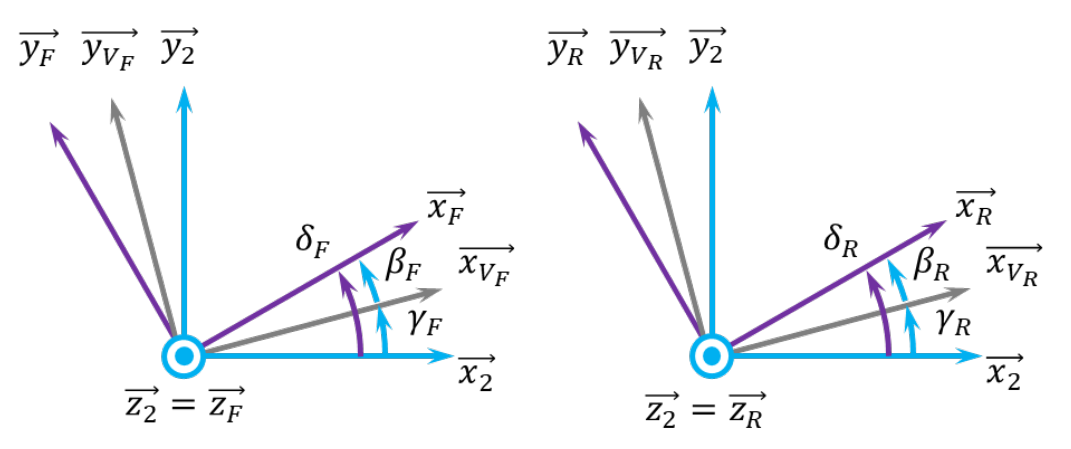
\includegraphics[width=0.9\linewidth]{img/figcor2}
\end{minipage}
}

\reponse{4}{}{
$\left \{
\begin{array}{rcl}
\vec{V}_{F,2/0}=V_F\cdot \vec{x}_{V_F}=V_F\cdot (cos(\theta+\gamma_F)\cdot\vec{x}_0+sin(\theta+\gamma_F)\cdot\vec{y}_0)\\
\vec{V}_{R,2/0}=V_R\cdot \vec{x}_{V_R}=V_R\cdot (cos(\theta+\gamma_R)\cdot\vec{x}_0+sin(\theta+\gamma_R)\cdot\vec{y}_0)
\end{array}
\right.$
}

\reponse{3}{}{
$\left \{
\begin{array}{rcl}
\dot{y}_F=-V_F\cdot sin(\theta+\gamma_F)\\
\dot{y}_R=-V_R\cdot sin(\theta+\gamma_R)
\end{array}
\right.$

Comme $\gamma_F=\delta_F-\beta_F$ et $\gamma_R=\delta_R-\beta_R$, on en déduit

$\left \{
\begin{array}{rcl}
\dot{y}_F=-V_F\cdot sin(\theta+\delta_F-\beta_F)\\
\dot{y}_R=-V_R\cdot sin(\theta+\delta_R-\beta_R)
\end{array}
\right.$
}

\ifdef{\public}{\newpage}

\reponse{5}{}{
$\vec{V}_{G_2,2/0}=\dot{x}_{G_2}\cdot \vec{x}_0-\dot{y}_{G_2}\cdot \vec{y}_0$

$\vec{V}_{G_2,2/0}=V_{G_2}\cdot \vec{x}_{V_{G_2}}=V_{G_2}\cdot (cos(\theta+\gamma_{G_2})\cdot\vec{x}_0+sin(\theta+\gamma_{G_2})\cdot\vec{y}_0)$

$\dot{x}_{G_2}=V_{G_2}\cdot cos(\theta+\gamma_{G_2})$
}

\reponse{2}{}{
$\vec{V}_{G_2,2/0}=\vec{V}_{F,2/0}+\overrightarrow{G_2F}\wedge\vec{\Omega}_{2/0}$
}

\reponse{4}{}{
$\overrightarrow{G_2F}=L\cdot\vec{x}_2$, donc $\overrightarrow{G_2F}\wedge\vec{\Omega}_{2/0}$ est perpendiculaire à $\vec{x}_2$, donc $\left(\overrightarrow{G_2F}\wedge\vec{\Omega}_{2/0}\right)\cdot\vec{x}_2=0$.
}

\reponse{4}{}{
$\vec{V}_{G_2,2/0}\cdot\vec{x}_2=\vec{V}_{F,2/0}\cdot\vec{x}_2+\overrightarrow{G_2F}\wedge\vec{\Omega}_{2/0}\cdot\vec{x}_2=\vec{V}_{F,2/0}\cdot\vec{x}_2$

On en déduira de même que $\vec{V}_{G_2}\cdot\vec{x}_2=\vec{V}_{F}\cdot\vec{x}_2=\vec{V}_{R}\cdot\vec{x}_2$
}

\ifdef{\public}{\newpage}

\reponse{5}{}{
$\vec{V}_{G_2,2/0}\cdot\vec{x}_2=V_{G_2}\cdot \vec{x}_{V_{G_2}}\cdot\vec{x}_2=V_{G_2}\cdot cos(\gamma_{G_2})$

De même, $\vec{V}_{F,2/0}\cdot\vec{x}_2=V_F\cdot cos(\gamma_F)$
et $\vec{V}_{R,2/0}\cdot\vec{x}_2=V_R\cdot cos(\gamma_R)$

Donc, $V_{G_2}\cdot cos(\gamma_{G_2})=V_F\cdot cos(\gamma_F)=V_R\cdot cos(\gamma_R)$
}

\reponse{7}{}{
Question 13: 

$\left \{
\begin{array}{rcl}
\dot{y}_F=-V_F\cdot sin(\theta+\delta_F-\beta_F) \rightarrow \dot{y}_F=-V_F\cdot(\theta+\delta_F-\beta_F)\\
\dot{y}_R=-V_R\cdot sin(\theta+\delta_R-\beta_R) \rightarrow \dot{y}_R=-V_R\cdot(\theta+\delta_R-\beta_R)
\end{array}
\right.$

Question 14:$\dot{x}_{G_2}=V_{G_2}\cdot cos(\theta+\gamma_{G_2}) \rightarrow \dot{x}_{G_2}=V_{G_2}$

Question 18: $V_{G_2}\cdot cos(\gamma_{G_2})=V_F\cdot cos(\gamma_F)=V_R\cdot cos(\gamma_R) \rightarrow V_{G_2}=V_F=V_R$

Donc, 

$\left \{
\begin{array}{rcl}
\dot{x}_{G_2}&=&V_{G_2}\\
\dot{y}_F&=&-V_{G_2}\cdot (\theta+\delta_F-\beta_F)\\
\dot{y}_R&=&-V_{G_2}\cdot (\theta+\delta_R-\beta_R)
\end{array}
\right.$
}

\reponse{6}{}{
Les premiers déterminent directement la position angulaire alors que les second compte le nombre d'incréments entre une position initiale (à déterminer).
}

\reponse{5}{}{
$\left \{
\begin{array}{rcl}
\dot{y}_F&=&-V_{G_2}\cdot (\theta+\delta_F-\beta_F)\\
\dot{y}_R&=&-V_{G_2}\cdot (\theta+\delta_R-\beta_R)
\end{array}
\right.$

Donc,

$\left \{
\begin{array}{rcl}
\widehat{\beta}_F&=&\frac{\dot{y}_F}{V_{G_2}}+\theta+\delta_F\\
\widehat{\beta}_R&=&\frac{\dot{y}_R}{V_{G_2}}+\theta+\delta_R
\end{array}
\right.$
}

\reponse{1}{\begin{center}
\begin{tabular}{|>{\centering\arraybackslash}p{1cm}|>{\centering\arraybackslash}p{1cm}|>{\centering\arraybackslash}p{1cm}|>{\centering\arraybackslash}p{1cm}|>{\centering\arraybackslash}p{1cm}|>{\centering\arraybackslash}p{1cm}|}

\hline
t & $\dot{y}_F$ & $V_{G_2}$ & $\theta$ & $\delta_F$ & $\widehat{\beta}_F$\\
\hline
0 & & & & & \\
\hline
1 & & & & & \\
\hline
2 & & & & & \\
\hline
3 & & & & & \\
\hline
4 & & & & & \\
\hline
5 & & & & & \\
\hline
\end{tabular}

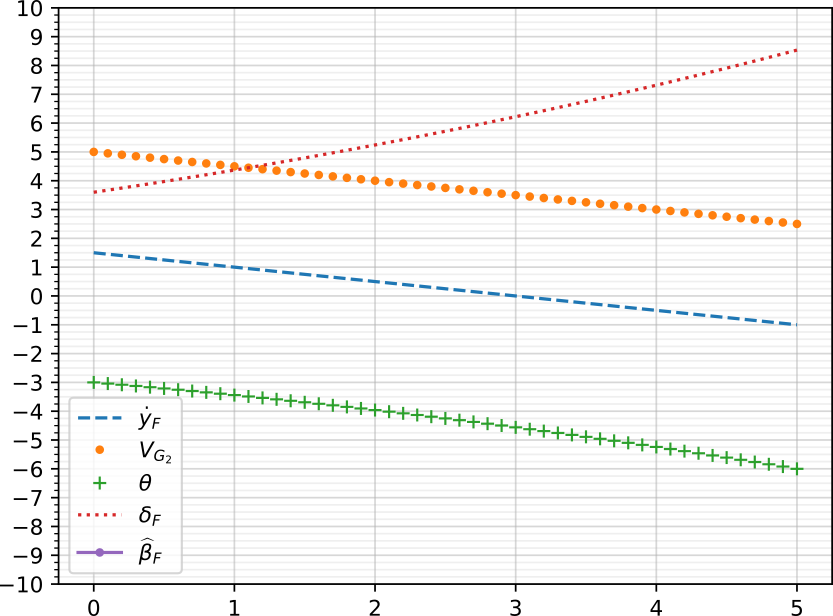
\includegraphics[width=0.7\linewidth]{img/figDR1}
\end{center}
}{
\begin{center}
\begin{tabular}{|>{\centering\arraybackslash}p{1cm}|>{\centering\arraybackslash}p{1cm}|>{\centering\arraybackslash}p{1cm}|>{\centering\arraybackslash}p{1cm}|>{\centering\arraybackslash}p{1cm}|>{\centering\arraybackslash}p{1cm}|}

\hline
t & $\dot{y}_F$ & $V_{G_2}$ & $\theta$ & $\delta_F$ & $\widehat{\beta}_F$\\
\hline
0 &  1.5 & 5.0 & -3.00 & 3.6 & 0.9 \\
\hline
1 & 1.0 & 4.5 & -3.44 & 4.37 & 1.15 \\
\hline
2 & 0.5 & 4.0 & -3.96 & 5.24 & 1.4 \\
\hline
3 & 0.0 & 3.5 & -4.56 & 6.22 & 1.66 \\
\hline
4 & -0.5 & 3.0 & -5.24 & 7.32 & 1.91 \\
\hline
5 & -1.0 & 2.5 & -6 & 8.53 & 2.13 \\
\hline
\end{tabular}

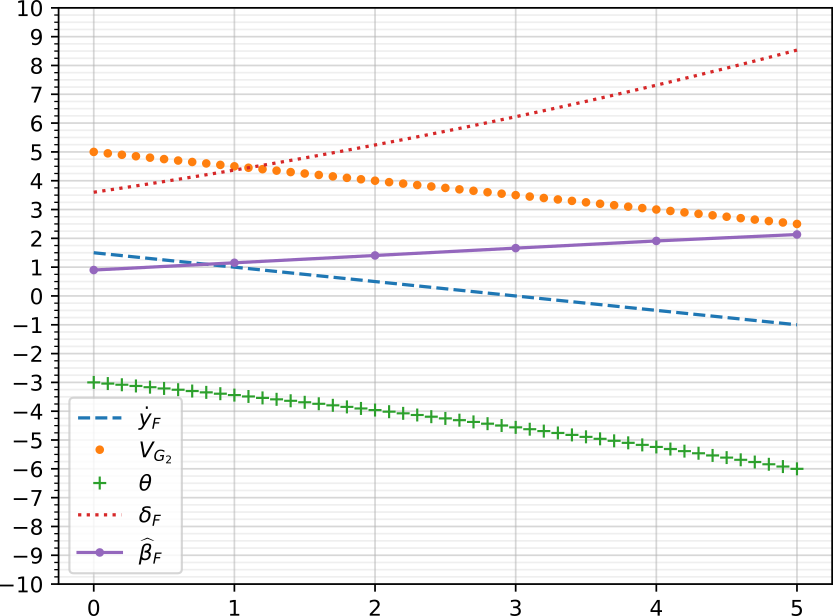
\includegraphics[width=0.7\linewidth]{img/figDR1_cor}
\end{center}
}

\ifdef{\public}{\newpage}

\reponse{3}{}{
Les angles étant tous faibles, l'hypothèse peut être utilisée.
}

\reponse{6}{}{
En se plaçant dans le quadrilatère $O_3O_1AB$ et en écrivant la fermeture géométrique, on a 
$\overrightarrow{O_3O_1} + \overrightarrow{O_1A} + \overrightarrow{AB} + \overrightarrow{BO_3}  = \vec{0}$\\
$-a \vec{x}_2 + b\vec{y}_2 -l_1 \vec{x}_1 -l_4 \vec{y}_4 + l_3 \vec{x}_3 = \vec{0}$.

Dans $\mathcal{B}_2$, on obtient:\\
$-a \vec{x}_2 + b\vec{y}_2 -l_1 \left(\cos\theta_{10} \vec{x}_2 + \sin\theta_{10} \vec{y}_2  \right)-l_4 \left( 
\cos \theta_{40} \vec{y}_2 - \sin\theta_{40} \vec{x}_2 \right) + l_3 \left(\cos\theta_{30} \vec{x}_2 + \sin\theta_{30} \vec{y}_2  \right)= \vec{0}$.

Donc  :
$
\left\{ 
\begin{array}{l}
-a  -l_1 \cos\theta_{10} + l_4   \sin\theta_{40}   + l_3 \cos\theta_{30} = 0 \\
 b -l_1  \sin\theta_{10} -l_4  \cos \theta_{40}  + l_3  \sin\theta_{30}   =0
\end{array}
\right.
$.

}

\reponse{6}{}{
$\left \{
\begin{array}{rcl}
l_3 \cos\theta_{30}&=&a   +l_1  \cos\theta_{10} -  l_4  \sin\theta_{40}     \\
l_3  \sin\theta_{30}&=&- b +l_1  \sin\theta_{10} + l_4  \cos \theta_{40}   \end{array}
\right.$

On utilise le fait que $\cos^2\theta_{30}+\sin^2\theta_{30}=1$.

$\left(a   +l_1  \cos\theta_{10} -  l_4  \sin\theta_{40} \right)^2 + 
\left(- b +l_1  \sin\theta_{10} + l_4  \cos \theta_{40}\right)^2 = l_3^2$ que l'on développe:

$a^2   +l_1^2  \cos^2\theta_{10} +  l_4^2  \sin^2\theta_{40} 
+ 2al_1\cos\theta_{10} - 2a  l_4  \sin\theta_{40} - 2l_1l_4 \cos\theta_{10}\sin\theta_{40}
+b^2 + l_1^2  \sin^2\theta_{10} + l_4 ^2 \cos^2 \theta_{40}
- 2bl_1  \sin\theta_{10} - 2b l_4  \cos \theta_{40} + l_1  \sin\theta_{10}l_4  \cos \theta_{40}  = l_3^2$ 

$a^2+ 2al_1\cos\theta_{10} - 2a  l_4  \sin\theta_{40} - 2l_1l_4 \cos\theta_{10}\sin\theta_{40}
+b^2 + l_1^2  + l_4 ^2 - 2bl_1  \sin\theta_{10} - 2b l_4  \cos \theta_{40} + l_1  \sin\theta_{10}l_4  \cos \theta_{40}  = l_3^2$ 

$-\sin\theta_{40}\left( 2a  l_4  + 2l_1l_4 \cos\theta_{10}\right)  
-\cos \theta_{40}\left( 2b l_4   - l_1  \sin\theta_{10}l_4  \right)
+a^2  + 2al_1\cos\theta_{10}  +b^2 + l_1^2  + l_4 ^2 - 2bl_1  \sin\theta_{10}   - l_3^2 = 0$.

Ainsi : 
$\left \{
\begin{array}{rcl}
 f_1\left(\theta_{10}\right) =a^2  + 2al_1\cos\theta_{10}  +b^2 + l_1^2  + l_4 ^2 - 2bl_1  \sin\theta_{10}   - l_3^2  \\
 f_2\left(\theta_{10}\right) =2a  l_4  + 2l_1l_4 \cos\theta_{10} \\
 f_3\left(\theta_{10}\right) = 2b l_4   - l_1  \sin\theta_{10}l_4 
\end{array}
\right.
$.
}

\ifdef{\public}{\newpage}

\reponse{1}{\begin{center}
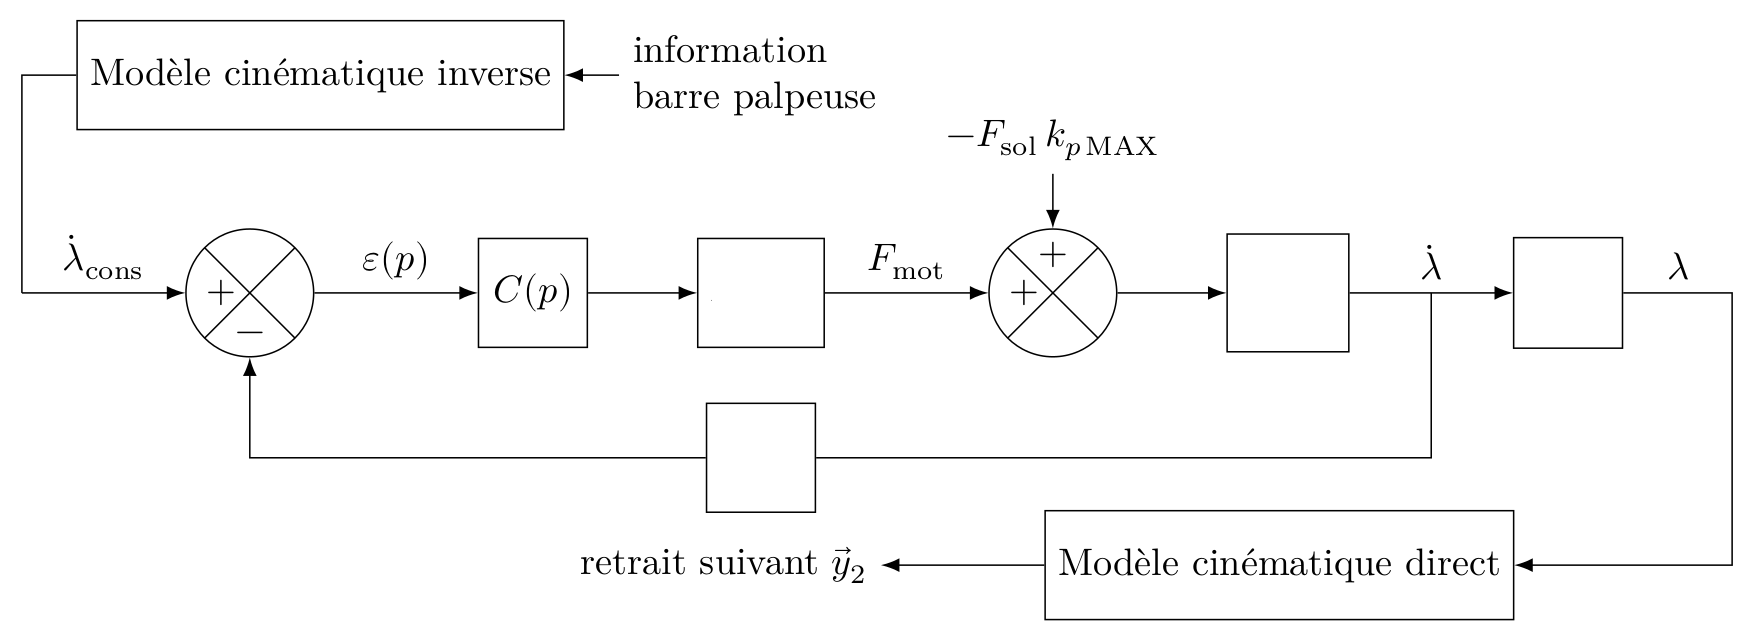
\includegraphics[width=0.8\linewidth]{img/fig10}
\end{center}}{
\begin{center}
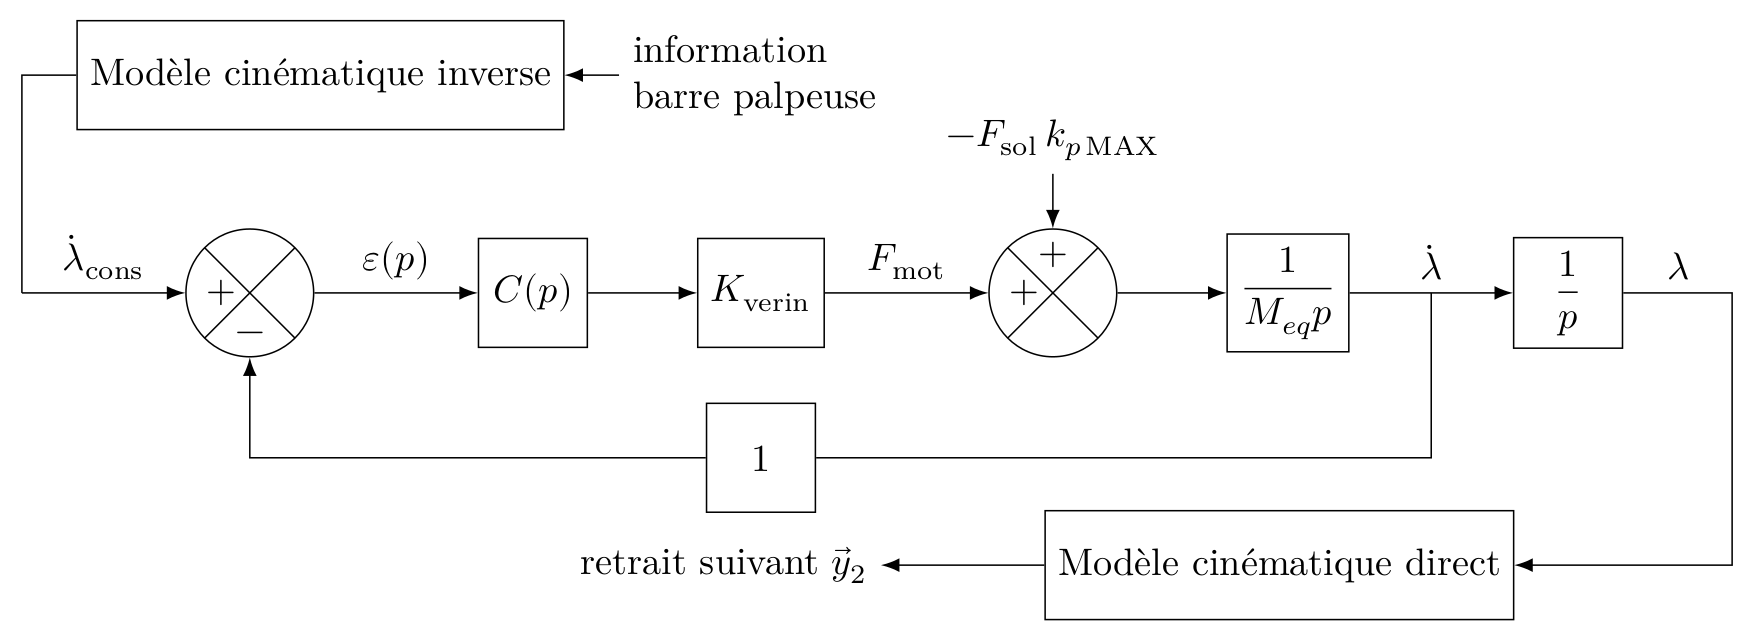
\includegraphics[width=0.8\linewidth]{img/fig10_cor}
\end{center}}


\reponse{6}{}{
$\dot{\lambda}=\frac{1}{M_{eq}\cdot p}\cdot(F_{mot}-F_{sol}\cdot k_{p\ MAX})$

$\dot{\lambda}=\frac{1}{M_{eq}\cdot p}\cdot(\varepsilon(p)\cdot K_c \cdot K_{verin}-F_{sol}\cdot k_{p\ MAX})$

$\dot{\lambda}=\frac{1}{M_{eq}\cdot p}\cdot((\dot{\lambda}_{cons}-\dot{\lambda})\cdot K_c \cdot K_{verin}-F_{sol}\cdot k_{p\ MAX})$

$\dot{\lambda}=\frac{1}{M_{eq}\cdot p}\cdot(\dot{\lambda}_{cons}\cdot K_c \cdot K_{verin}-F_{sol}\cdot k_{p\ MAX})-\frac{1}{M_{eq}\cdot p}\cdot\dot{\lambda}\cdot K_c\cdot K_{verin}$

$\dot{\lambda}\cdot\left(1+\frac{1}{M_{eq}\cdot p}\cdot K_c\cdot K_{verin}\right)=\frac{1}{M_{eq}\cdot p}\cdot(\dot{\lambda}_{cons}\cdot K_c \cdot K_{verin}-F_{sol}\cdot k_{p\ MAX})$

$\dot{\lambda}=\frac{\frac{1}{M_{eq}\cdot p}\cdot K_c \cdot K_{verin}}{1+\frac{1}{M_{eq}\cdot p}\cdot K_c\cdot K_{verin}}\cdot\dot{\lambda}_{cons}+
\frac{\frac{1}{M_{eq}\cdot p}}{1+\frac{1}{M_{eq}\cdot p}\cdot K_c\cdot K_{verin}}\cdot \left(-F_{sol}\cdot k_{p\ MAX}\right)$

Ainsi, 

$H_1(p)=\frac{\frac{1}{M_{eq}\cdot p}\cdot K_c \cdot K_{verin}}{1+\frac{1}{M_{eq}\cdot p}\cdot K_c\cdot K_{verin}}=\frac{K_c \cdot K_{verin}}{M_{eq}\cdot p+K_c\cdot K_{verin}}=\frac{1}{1+\frac{M_{eq}}{K_c\cdot K_{verin}}\cdot p}$

$H_2(p)=\frac{1}{M_{eq}\cdot p+K_c\cdot K_{verin}}=\frac{\frac{1}{K_c\cdot K_{verin}}}{1+\frac{M_{eq}}{K_c\cdot K_{verin}}\cdot p}$
}

\reponse{6}{}{
$\frac{M_{eq}}{K_c\cdot K_{verin}}=\frac{M}{F\cdot L^{-1}\cdot T}=\frac{M}{M\cdot L\cdot T^{-2} \cdot L^{-1}\cdot T}=\frac{1}{T^{-1}}=T$

C'était prévisible car il s'agit du $\tau$ du dénominateur de la fonction de transfert.
}

\reponse{10}{\begin{center}
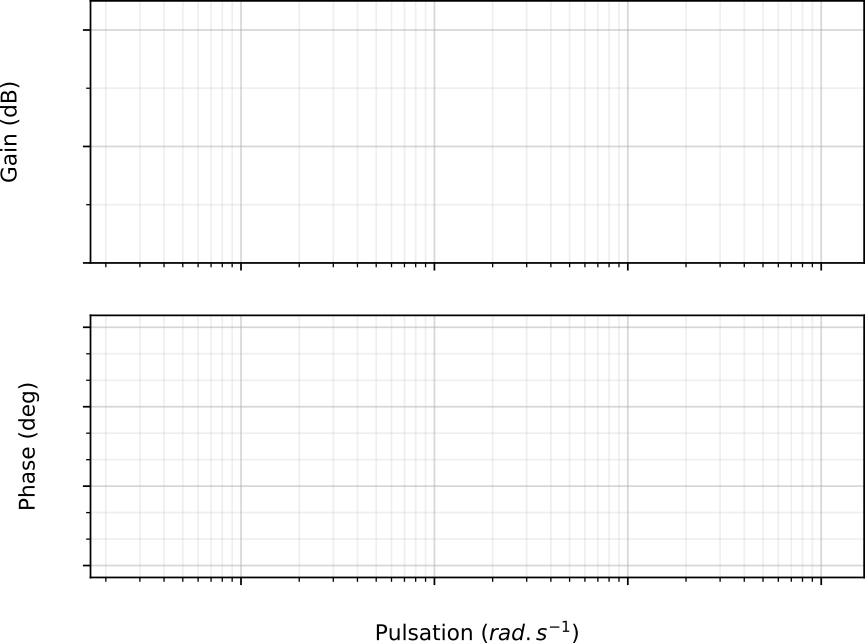
\includegraphics[width=0.8\linewidth]{img/Bode}
\end{center}}{
\begin{center}
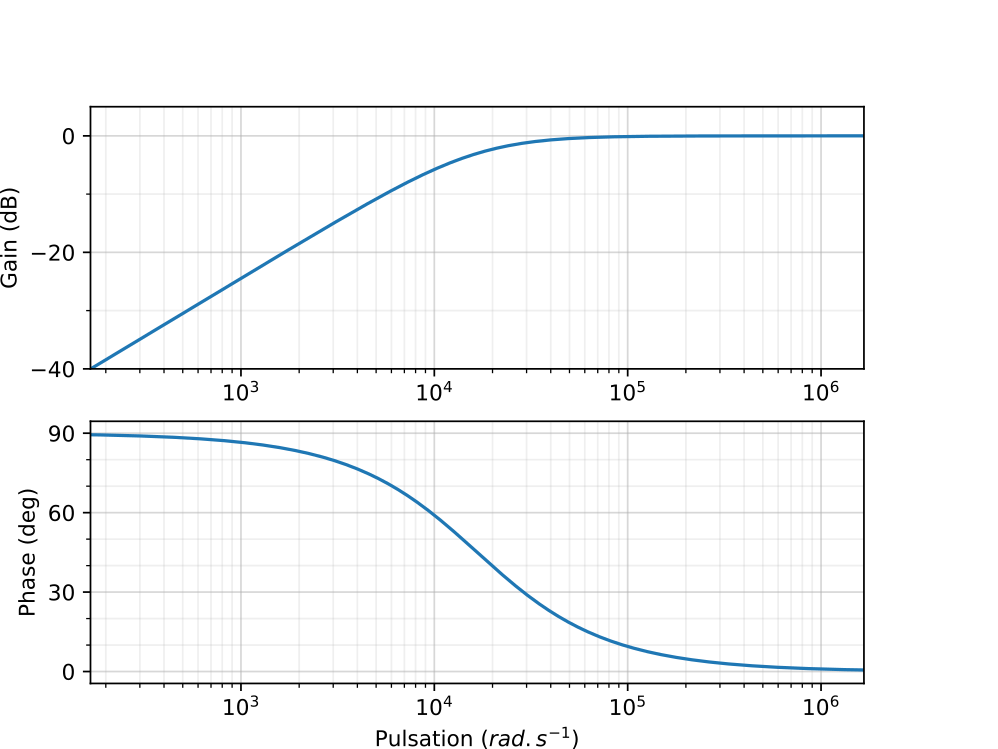
\includegraphics[width=0.8\linewidth]{img/Bode_cor}
\end{center}}

\ifdef{\public}{\newpage}

\reponse{1}{\begin{center}
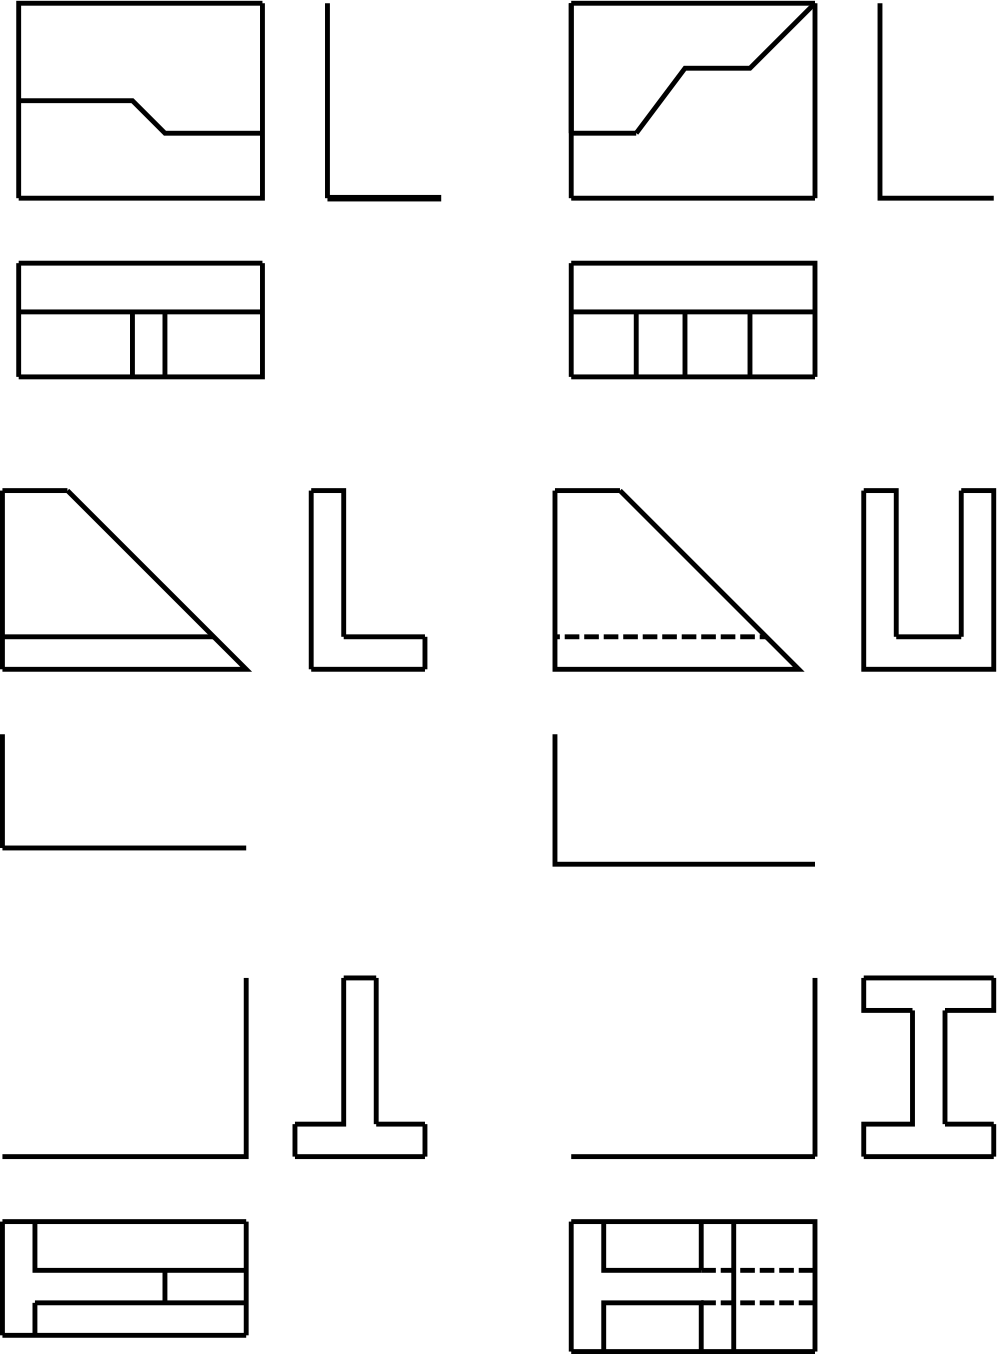
\includegraphics[width=0.8\linewidth]{img/DR_dessin}
\end{center}}{
\begin{center}
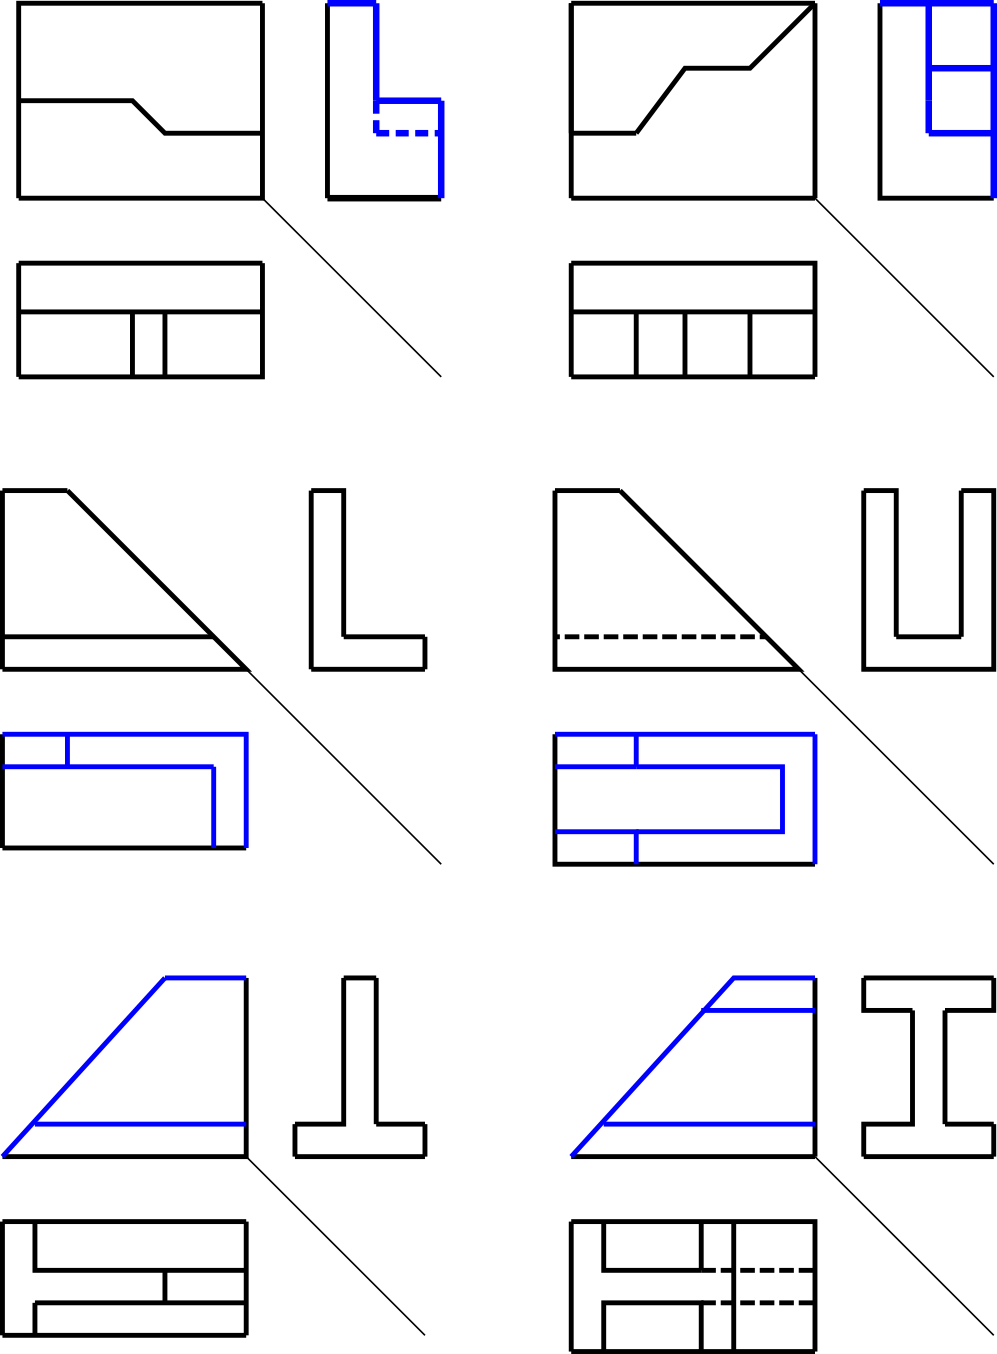
\includegraphics[width=0.8\linewidth]{img/DR_dessin_cor}
\end{center}}

\end{document}

